
%% Add the 'procedia' option to approximate to the Word template
\documentclass[3p,procedia]{elsarticle}
\usepackage{ecrc}
\usepackage{color,soul}
\usepackage{multirow}
\usepackage{booktabs}
\graphicspath{{images/}}
\usepackage{lscape}
\usepackage{amssymb}
\usepackage{lineno}
\usepackage{hyperref}
\usepackage{subfig}
\usepackage[export]{adjustbox}

\volume{00}
\firstpage{1}
%\journalname{Forest ecology and management}
\runauth{Gilles A. et al.}

\DeclareUnicodeCharacter{00E4}{\"a}% pour -niittyla

\begin{document}

\begin{frontmatter}

\author[label1]{Gilles Arthur}
\ead{arthur.gilles@uliege.be}
\author[label1]{Lisein Jonathan}
\author[label2]{Lemaire Jean}
\author[label2]{Cansel Juliette}
\author[label3]{Piedallu Christian}
\author[label1]{Claessens Hugues}

\fntext[label1]{Liège University - Faculty of Gembloux Agro-Bio Tech - unit of forest ressources managment}
\fntext[label2]{Centre National de la propriété forestière}
\fntext[label3]{Université de Lorraine, AgroParisTech, Inra, Silva, F-54000 Nancy, AgroParisTech, 14 rue Girardet, F-54042 Nancy Cedex, France}


\dochead{Original research papers}

\title{Spruce vulnerability to bark beetle attack vary with altitude and topographic position: a remote sensing analysis in Belgium and France}
\begin{abstract}
	
\iffalse
Following the droughts of 2018 to 2020, numerous Norway spruce diebacks were caused by bark beetles 
%(Ips typographus/ Pityogenes chalcographus)
outbreaks in Wallonia and in the Grand-Est. 
A methodology for detection the health status of spruce was developed based on satellite imagery from the European Union's Earth Observation Programme.
The time series of satellite images allowed the modelling of the spectral response of healthy spruce forests over the seasons. Deviations from this seasonal vegetation index trajectory for a healthy spruce stand are caused by a decrease in photosynthetic activity of the forest canopy.
This decrease in photosynthesis is caused by a bark beetle attack and is detected automatically.
This technique, inspired by the work of INRAe, is robust because of the redundancy of the information from the spatial images, which are repeated every 3-4 weeks. 
The method results in the production of annual maps of the health status of the Walloon and Grand-Est spruce forests.
The most important damage occurred in the years 2018-2019, affecting 2.8\% of the total area of spruce stands in Wallonia.
Although the main part of the crisis seems to be behind us, it remains to draw the necessary conclusions.
The relationship between climatic conditions and the presence of the bark beetle has proven to be complex in Wallonia.
Nevertheless, a very strong relationship between altitude and the presence of bark beetle damage could be demonstrated.
Stands below 300m in altitude were indeed much more affected.
Moreover, forest sites located on steep slopes ( $\ge$  20 \%), whether on cold or warm slopes, are more affected than sites located on low slopes (plateaus).
In the Grand-Est, the peak of the crisis has been reached in 2019-2020. Altitude and slopes are not strongly influencing factors for spruce dieback. 

\fi
\end{abstract}

\begin{keyword}
  Norway spuce \sep Species vulnerability \sep Bark Beetle \sep forest management \sep forest site \sep topographic condition \sep time series \sep Sentinel-2
\end{keyword}

\end{frontmatter}

\linenumbers

\section{Introduction}

Global changes are increasing the risk of disturbances in forest environment: frequency and intensity of abiotic (fire, storm, drough) and biotic (pest invasion) will be more recurrent \citep{lindner_climate_2010}.
In Western Europe, we expect a decrease of precipitation and a increase of drought events during the vegetation period, which will impact the actual geographic distribution of tree species \citep{hanewinkel2013climate}.
Due to the long time required to complete a forest revolutions, forest managers have to anticipate likely changes in climate conditions by modifying the forest tree species they used to regenerate at a particular location, in a way that the future environmental conditions of the forest site still meet the species requirements.
Norway spruce (\textit{Picea abies L. Karst}) is one of the most important economic plant species in Europe \citep{nystedt_norway_2013}.
Its productivity comes with a demanding amount of precipitation, thus making it sensitive to climate changes.
Plus, its major pest is bark beetle that cause important outbreak after storm, which provide breeding material e.g. windfalls, candle, or after severe drougth that weaken trees.
A recent bark beetle crisis, triggered by the exceptionally hot and dry weather of 2018, occurred in Western Europe and lasted until 2021. 
It has urged the need of adapting forest management practices. 
Indeed, forest practitioners have to decide now which species will replace Norway spruce in the thousands of clear-cutted hectares decimated by bark beetle attacks. 
The decision-making of replanting spruce requires a proper understanding of both Norway spruce and bark beetle autecology.

The Norway spruce is adapted to wide range of environmental conditions, although it prefers cold and humid climate.
It is naturally present in part of the Grand-Est (Vosges mountains) and artificially in Wallonia, where it was introduced during the second half of the 19th century \citep{Noirfalise_1975}.
The massive reforestations occurring at this time have led to the formation of large pure even-aged stands.
Moist and reasonably fertile soils are favourable for its productive cultivation \citep{horgan_guide_2003}.
It usually develops a taproot system with fine roots in shallow depth, although the roots go deeper on restrictive soil conditions \citep{puhe_roots_2003}.   
The precipitation are its primary water source \citep{tjoelker_outline_2007} and lack of water induces stress that affect growth and health of the tree. 
The most important pest for Norway spruce are bark beetles species.
The bark beetle species \textit{Ips typographus} causes the most important damages.
In this paper, bark beetle refers to the species \textit{Ips typographus}.
Stressed Norway spruce produce volatile compounds which attract bark beetles, making himself more susceptible to pest attack \citep{netherer_waterlimiting_2015,netherer_interactions_2021}.
Bark beetles are ubiquitous in the forest and their populations are usually low (endemic phasis).
Many stressed trees  cause a shift to an epidemic phasis with a explosion of bark beetle populations during which even healthy trees are massively attacked \citep{kautz_individual_2014}.
The life cycle of bark beetle depends on temperature and photoperiod \citep{baier_phenipscomprehensive_2007,annila_influence_1969}.
After spring swarming, the adult enter in the bark and burrow wood to make brood gallery where they mate and lay the eggs that mature to larvae int the phloem \citep{hlasny_bark_2021}.
In North Europe, the bark beetle is univoltine (one single generation) but it is multivoltine (breed two or even three generations) in Western and Central Europe \citep{annila_influence_1969}.
The bark beetle adult can re-emerge and swarm a second time to give birth to one sister brood \citep{zolubas_1995}.
After the larvae maturation that last about seven weeks, the new generation of beetles emerge and attack the direct surrounding trees \citep{zolubas_1995}.
Attacked trees defend themselves by pulsing resin to kill the bark beetle but these defence failed to resist again numerous simultaneous attacks that induce the decline and rapid death.
The Norway spruce dieback goes through three physiological stages which are denominated green, red and grey stage.
In the green stage, the bark beetle has succeeded to penetrate the phloem and the spruce retains its green needles. 
The tree is still alive but begins to suffer of water shortage cause by sap conduction problem. 
After several weeks, the red stage is reached when the needles turn brown-red. The tree is recently dead and the dry needles start to fall.
When all the needles of the spruce have fallen off and the grey bark of the trunk is visible, the grey stage is reached \citep{abdullah_european_2018}. 

To control the infestation of bark beetle, the solutions are limited. 
The use of phytosanitary product is forbidden in Belgian and French forest.
There is a pheromone trap system but it is not efficient to limit the damage in case of bark beetle outbreak \citep{kuhn_pheromone_2022}.
The only solution to limit the outbreak its to remove felled tree before the swarming to limit the presence of ideal breeding material and realize sanitary cutting when the tree is attacked by bark beetle at the green stage to decrease the bark beetle population. 

The European Union’s earth observation programme, with its satellite twin constellation Sentinel-2A and Sentinel-2B, provides free earth imagery with a high revisit time that have been intensively used for forestry purpose. 
Time series of Sentinel-2 (S2) images enable to model the phenology courses of vegetation indices in order to detect forest disturbances \citep{low_phenology_2020}, like the one caused by bark beetle outbreaks.
Infestation maps of the last sanitary crisis have been generated for Germany \citep{ali_canopy_2021,thonfeld_first_2022}, Czech Republic \citep{barta_early_2021}, Italy \citep{dalponte_mapping_2022} and France \citep{nardi_drought_2022}. 
This paper aims at studying the extent and the dynamic of the 2017-2021 bark beetle outbreak in Wallonia (Belgium) and in the Grand-Est (France).
To this end, we map Norway spruce dieback using S2 time series.
Then, we analyse the relationship between forest stands, bark beetle and environmental conditions in order to determine the most sensitive forest sites where Norway spruce should not be regenerated.


\section{Material and methods}
\subsection{Study area}
The study area was located in Wallonia (south of Belgium) and in the Grand-Est (north-east of France).

\begin{figure} [htbp] 
	\centering
	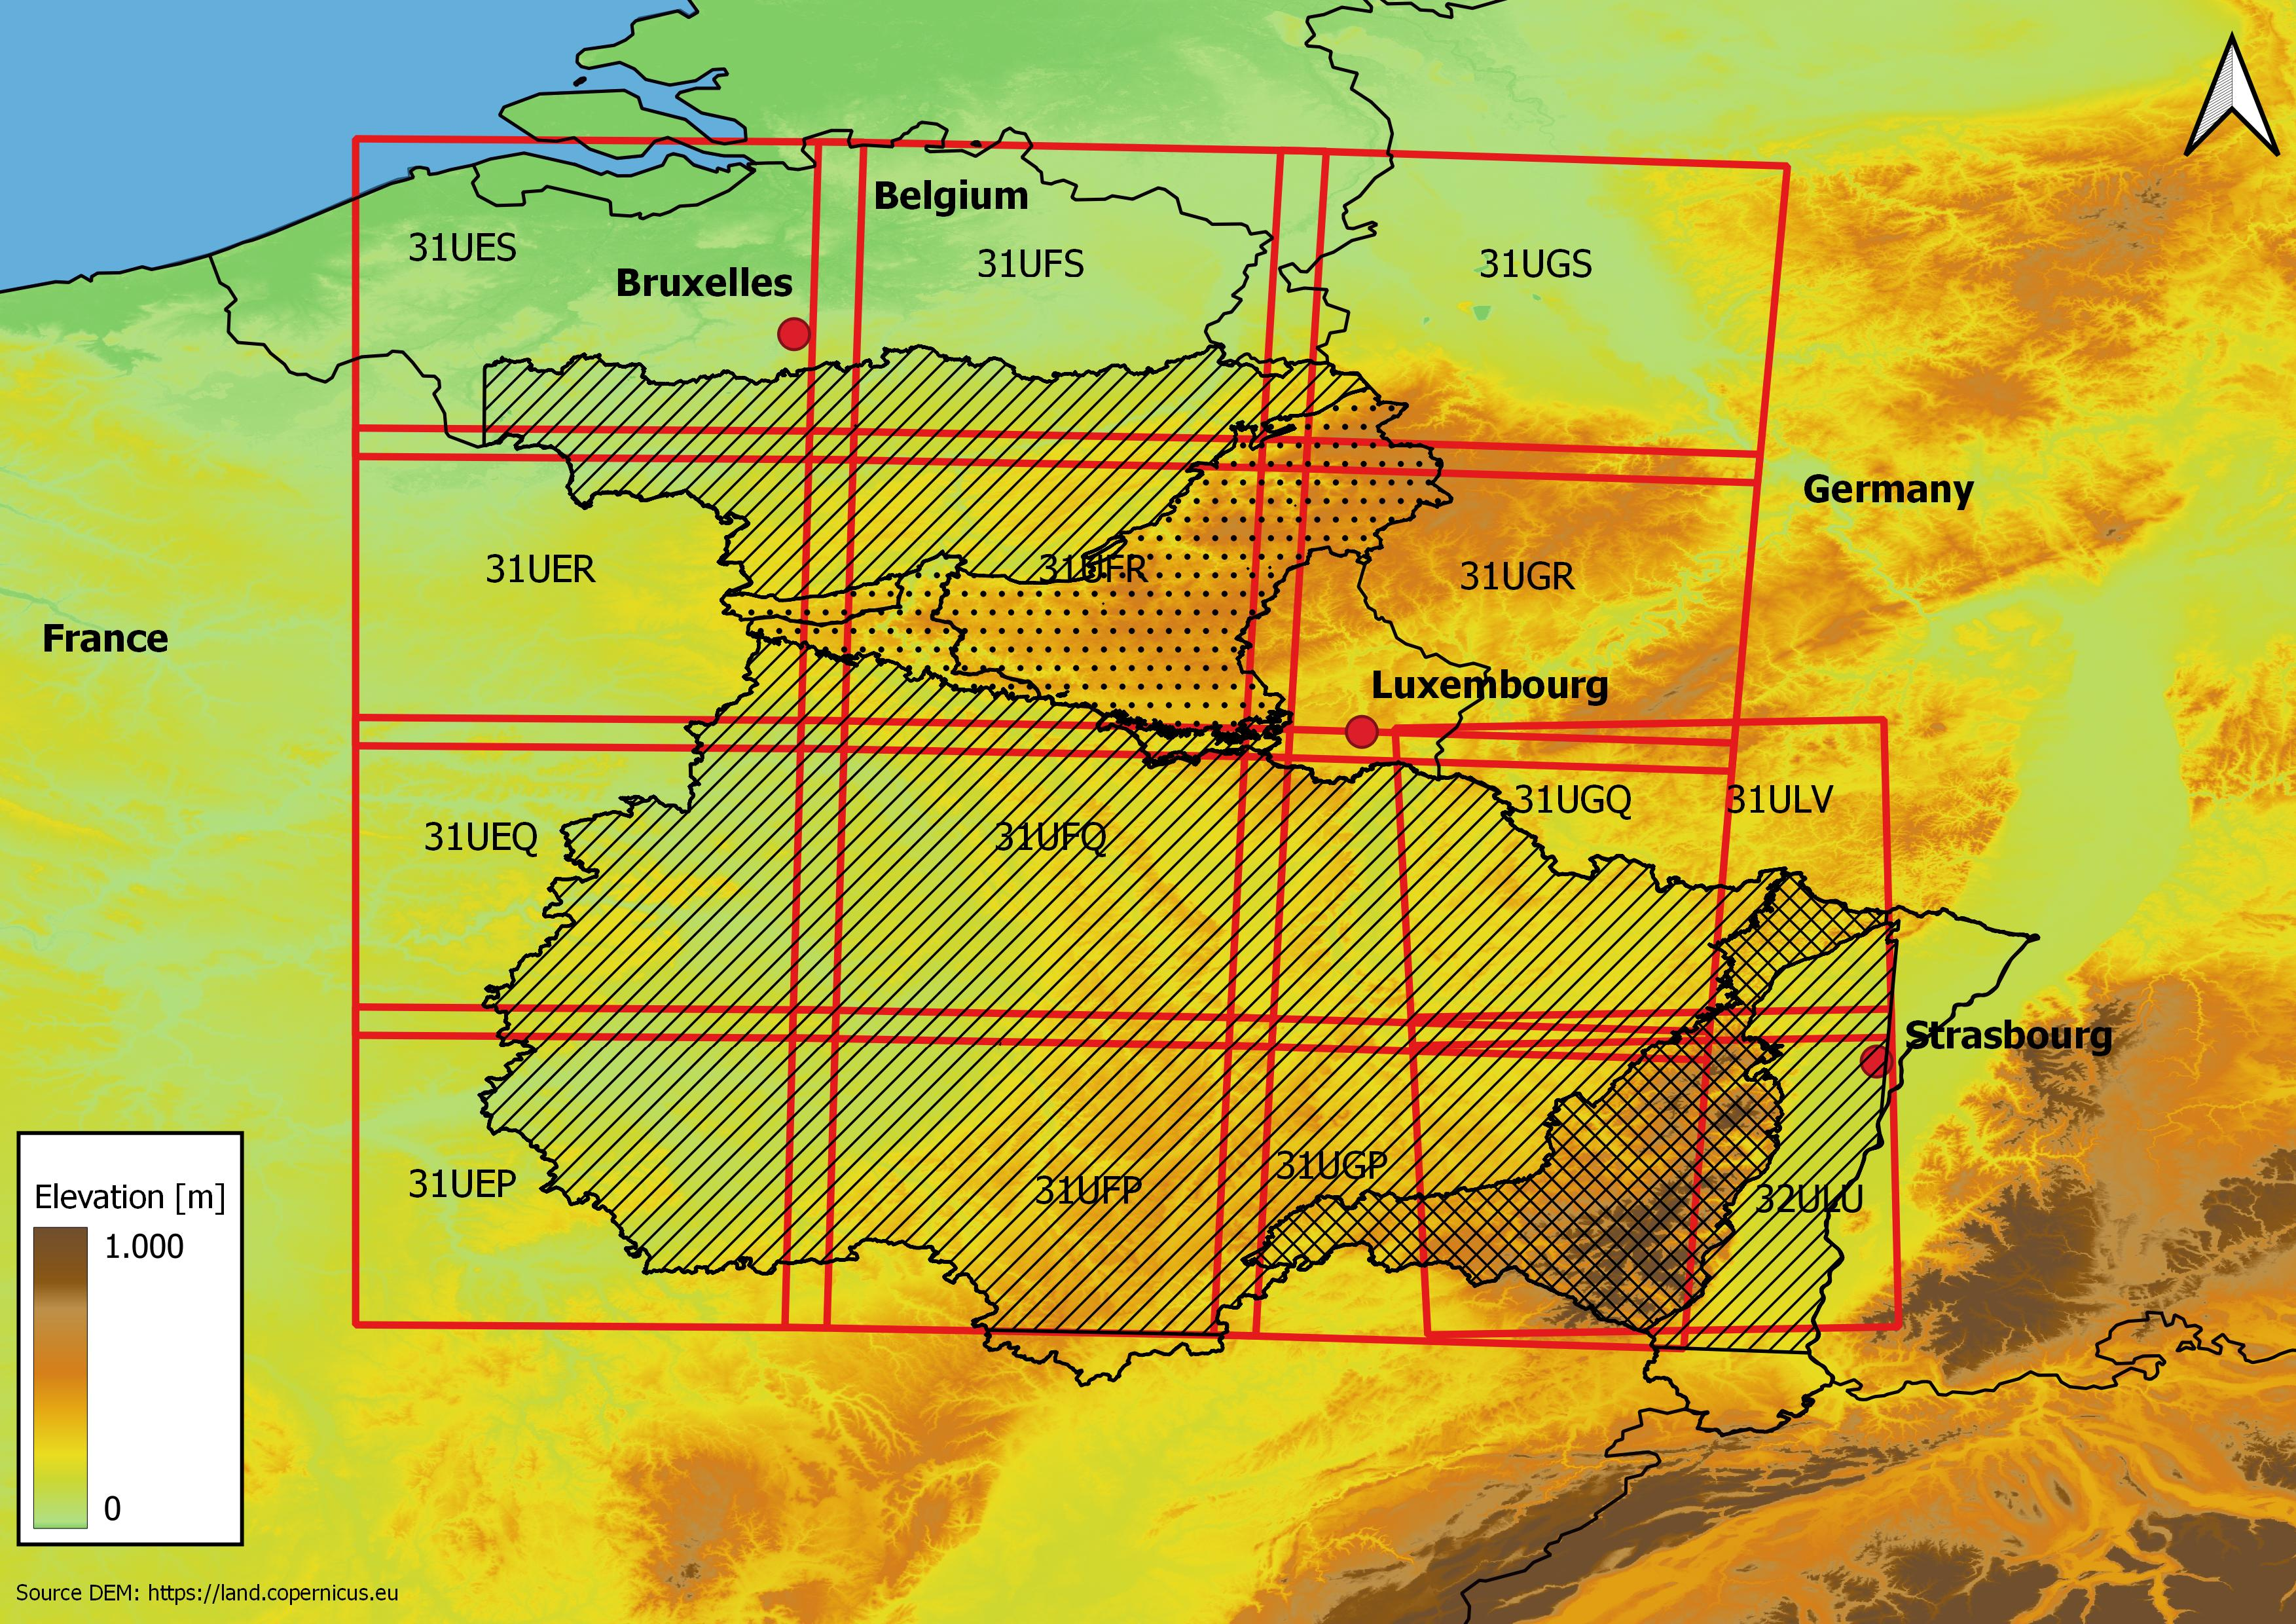
\includegraphics[width=0.8\textwidth]{gde.jpeg}
	\caption{Study area: Plains (hashed, altitude varying between 100 and 500 meters above see level), Ardenne (black dot, altitude between 100 and 700 m) and Vosges (cross, altitude ranging from 300 to 1300 m). Red squares illustrates the extend of Sentinel satellite 2 tiles which are used for the detection of bark beetle attack.}
	\label{fig:situ}
\end{figure}

The walloon forest covers 554 600 Ha. 
The Norway spruce stand occuped a quarter of Walloon forest \citep{Alderweireld_2015}. 
Two thirds of the Walloon spruce forest is located above 400m altitude. 
The Walloon climate is included in the temperate oceanic bioclimatic zone \citep{lindner_climate_2010}. 
The Grand-est forest occupies 1 939 000 ha. 
The Norway spruce covers seven percent of the forest of this region  \citep{IGN2022}. 
The majority of Norway spruce stand of this region grow between 400m and 900m. 
The Grand-est is included in the temperate oceanic bioclimatic zone\citep{lindner_climate_2010}. 

We have used the digital surface model data from the Copernicus Land Monitoring Service \citep{DEM_copernicus}  at a resolution of 25mX25m for all altitude data and slope calculations.
We determined the solar orientation using the \cite{Delvaux_galoux} definition of the three topography orientations.
Plateau and low slope are slope less than  20\% that does not create a particular micro-climate. 
North facing slopes are slopes greater than  20\% facing north. 
These are shady, cool and humid areas. 
South facing slopes are slope greater than  20\% facing south. 
In this orientation the air is warmer and drier and the temperature difference between day and night is greater.
Based on this definition and on the DEM, we produced topography orientation  maps for Wallonia and the Grand-Est.

%Solar orientation influences bark beetle capture in pheromone traps \citep{AFR64}.

Climate data for Wallonia have been provided by the Institut Royal Météorologique(IRM). The resolution of the data is 5km X 5km. Climate data of  Grand-est come from the data base Digitalis \citep{piedallu_presentation_2014}. The resolution of this data is 1km X 1km.

The French natural region and the Bioclimatic area of Wallonia have been grouped by average temperature and precipitation during the growing season  in three climatic areas: Ardenne, Plains and Vosges (Figure \ref{fig:clim}).
The Plains is a group of natural region with growing season temperature between 15.5°C and 18°C and with growing season  precipitation between 300mm and 400mm.

The Ardenne is defined a set of natural regions with a temperature of the growing season between 14°C and 15,5°C and a average precipitation during the growing season between 400m and 450 mm.
Vosges are natural regions with growing season temperature varies between 15.5°C and 17 °C and the growing season precipitation between 425mm and 600mm.
The figure \ref{fig:situ} show localisation of the three climatic areas in function of the altitude. 


\begin{figure}
	\centering
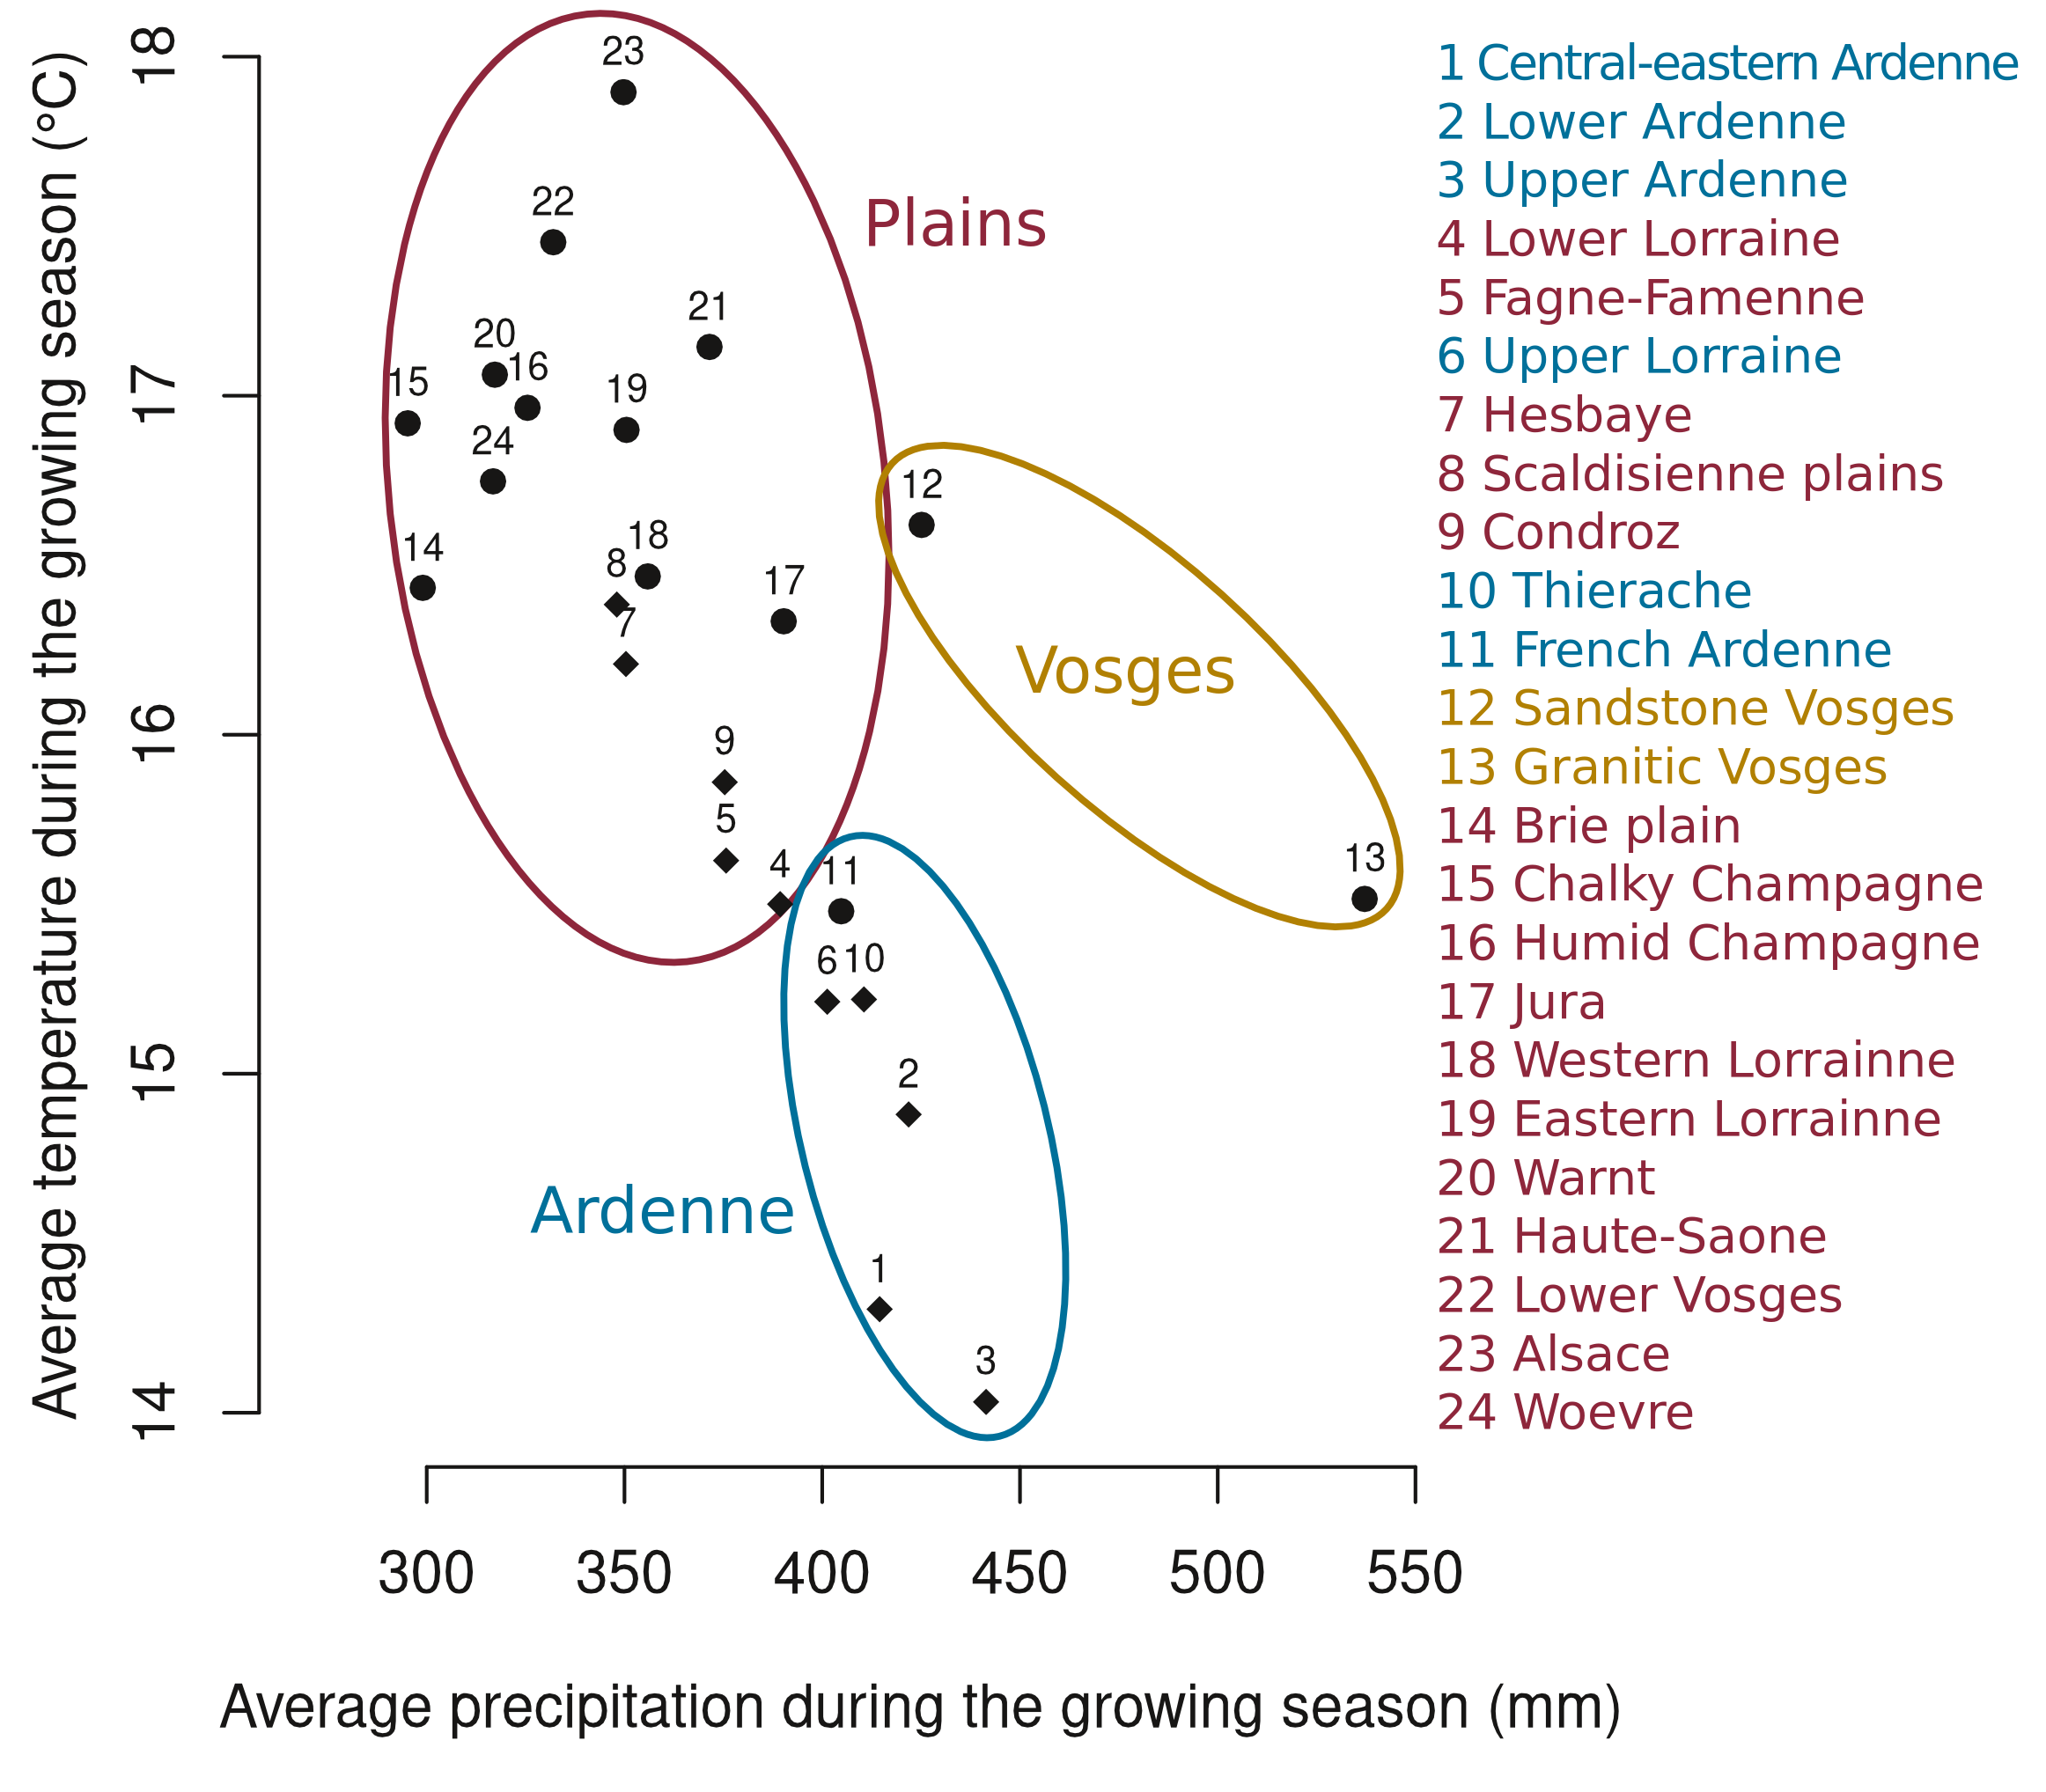
\includegraphics[width=0.8\linewidth]{climat/climat_region.png}
\caption{Grouping of French natural regions according to the temperature and precipitation of the growing season to form three groups: Ardenne (blue), Plains (red) and Vosges (orange). Wallonia natural regions are depicted with diamond-shaped points, and Grand-Est regions are illustrated by rounded points.}
	\label{fig:clim}
\end{figure}


%MNH

\subsection{Mapping of spruce dieback and mortality by analysis of sentinel-2 time-serie}


In the present research, the detection of bark beetle infestation is realized by using dense time series of S2 imagery following the methodology developped by \cite{dutrieux_package_2021}.
Sentinel-2 (S2) satellites carry multispectral sensor with a ground resolution up to 10 m.
The two regions  studied are covered by 14 Sentinel-2 tiles (Figure \ref{fig:situ}).  
Vegetation changes are tracked by means of a phenology metric, the \textit{SWIR Continuum Removal} ($SWIR_{CR}$) indice.
All S2 acquisitions are used in the analyses, provided that the cloud couver do not excess 35 percent. 
Bottom Of Atmosphere reflectance images (L2A product) are downloaded from the Theia data cluster \citep{theia_team} for all the 6 granules, which are tiles of 100km x 100km, that covers Wallonia. 
For north France, 10 granules cover the Grand-Est.
The $SWIR_{CR}$ is based on three spectral bands, the near-infrared, the shortwave infrared 1 band and the shortwave infrared 2, and is sensitive to the foliage water content (figure \ref{fig:harmo}).
Seasonal variation of $SWIR_{CR}$ for healthy stand is modelled and a bark beetle attack is detected if the observations deviates from the healthy phenology trajectory. 
Figure \ref{fig:harmo} illustrates a time-serie of $SWIR_{CR}$ observations (grey dots) for one pixel. 
In 2018, the observations goes beyond the threshold represented by the purple-dashed line, which shows that the spruce stand suffer from a serious stress induced by a bark beetle attack.
A bark beetle outbreak is confirmed as soon as $SWIR_{CR}$ vegetation indice show a stress for at least three consecutive times.
In parallel to the detection of bark beetle stress, stand cutting and thinning are subject of particular attention. 
Bare soil is detected by using a combination of red, green and shortwave infrared reflectance values.
Cutting are thus taken into account and are classified either as normal harvest cutting or as sanitary thinning based on the health status prior to the cutting.
The analysis of image time-serie is thus quite straightforward and is performed individually pixel per pixel starting from the 2016 year, which is the beginning of S2 acquisitions. 
The dense time-serie covers the 2016-2021 period and count a minimum of 180 acquistion dates. 
The health status is summarized in annual health maps by means of four classes ; healthy, bark beetle attached, cutted and sanitary thinning.

\begin{figure}
	\centering
	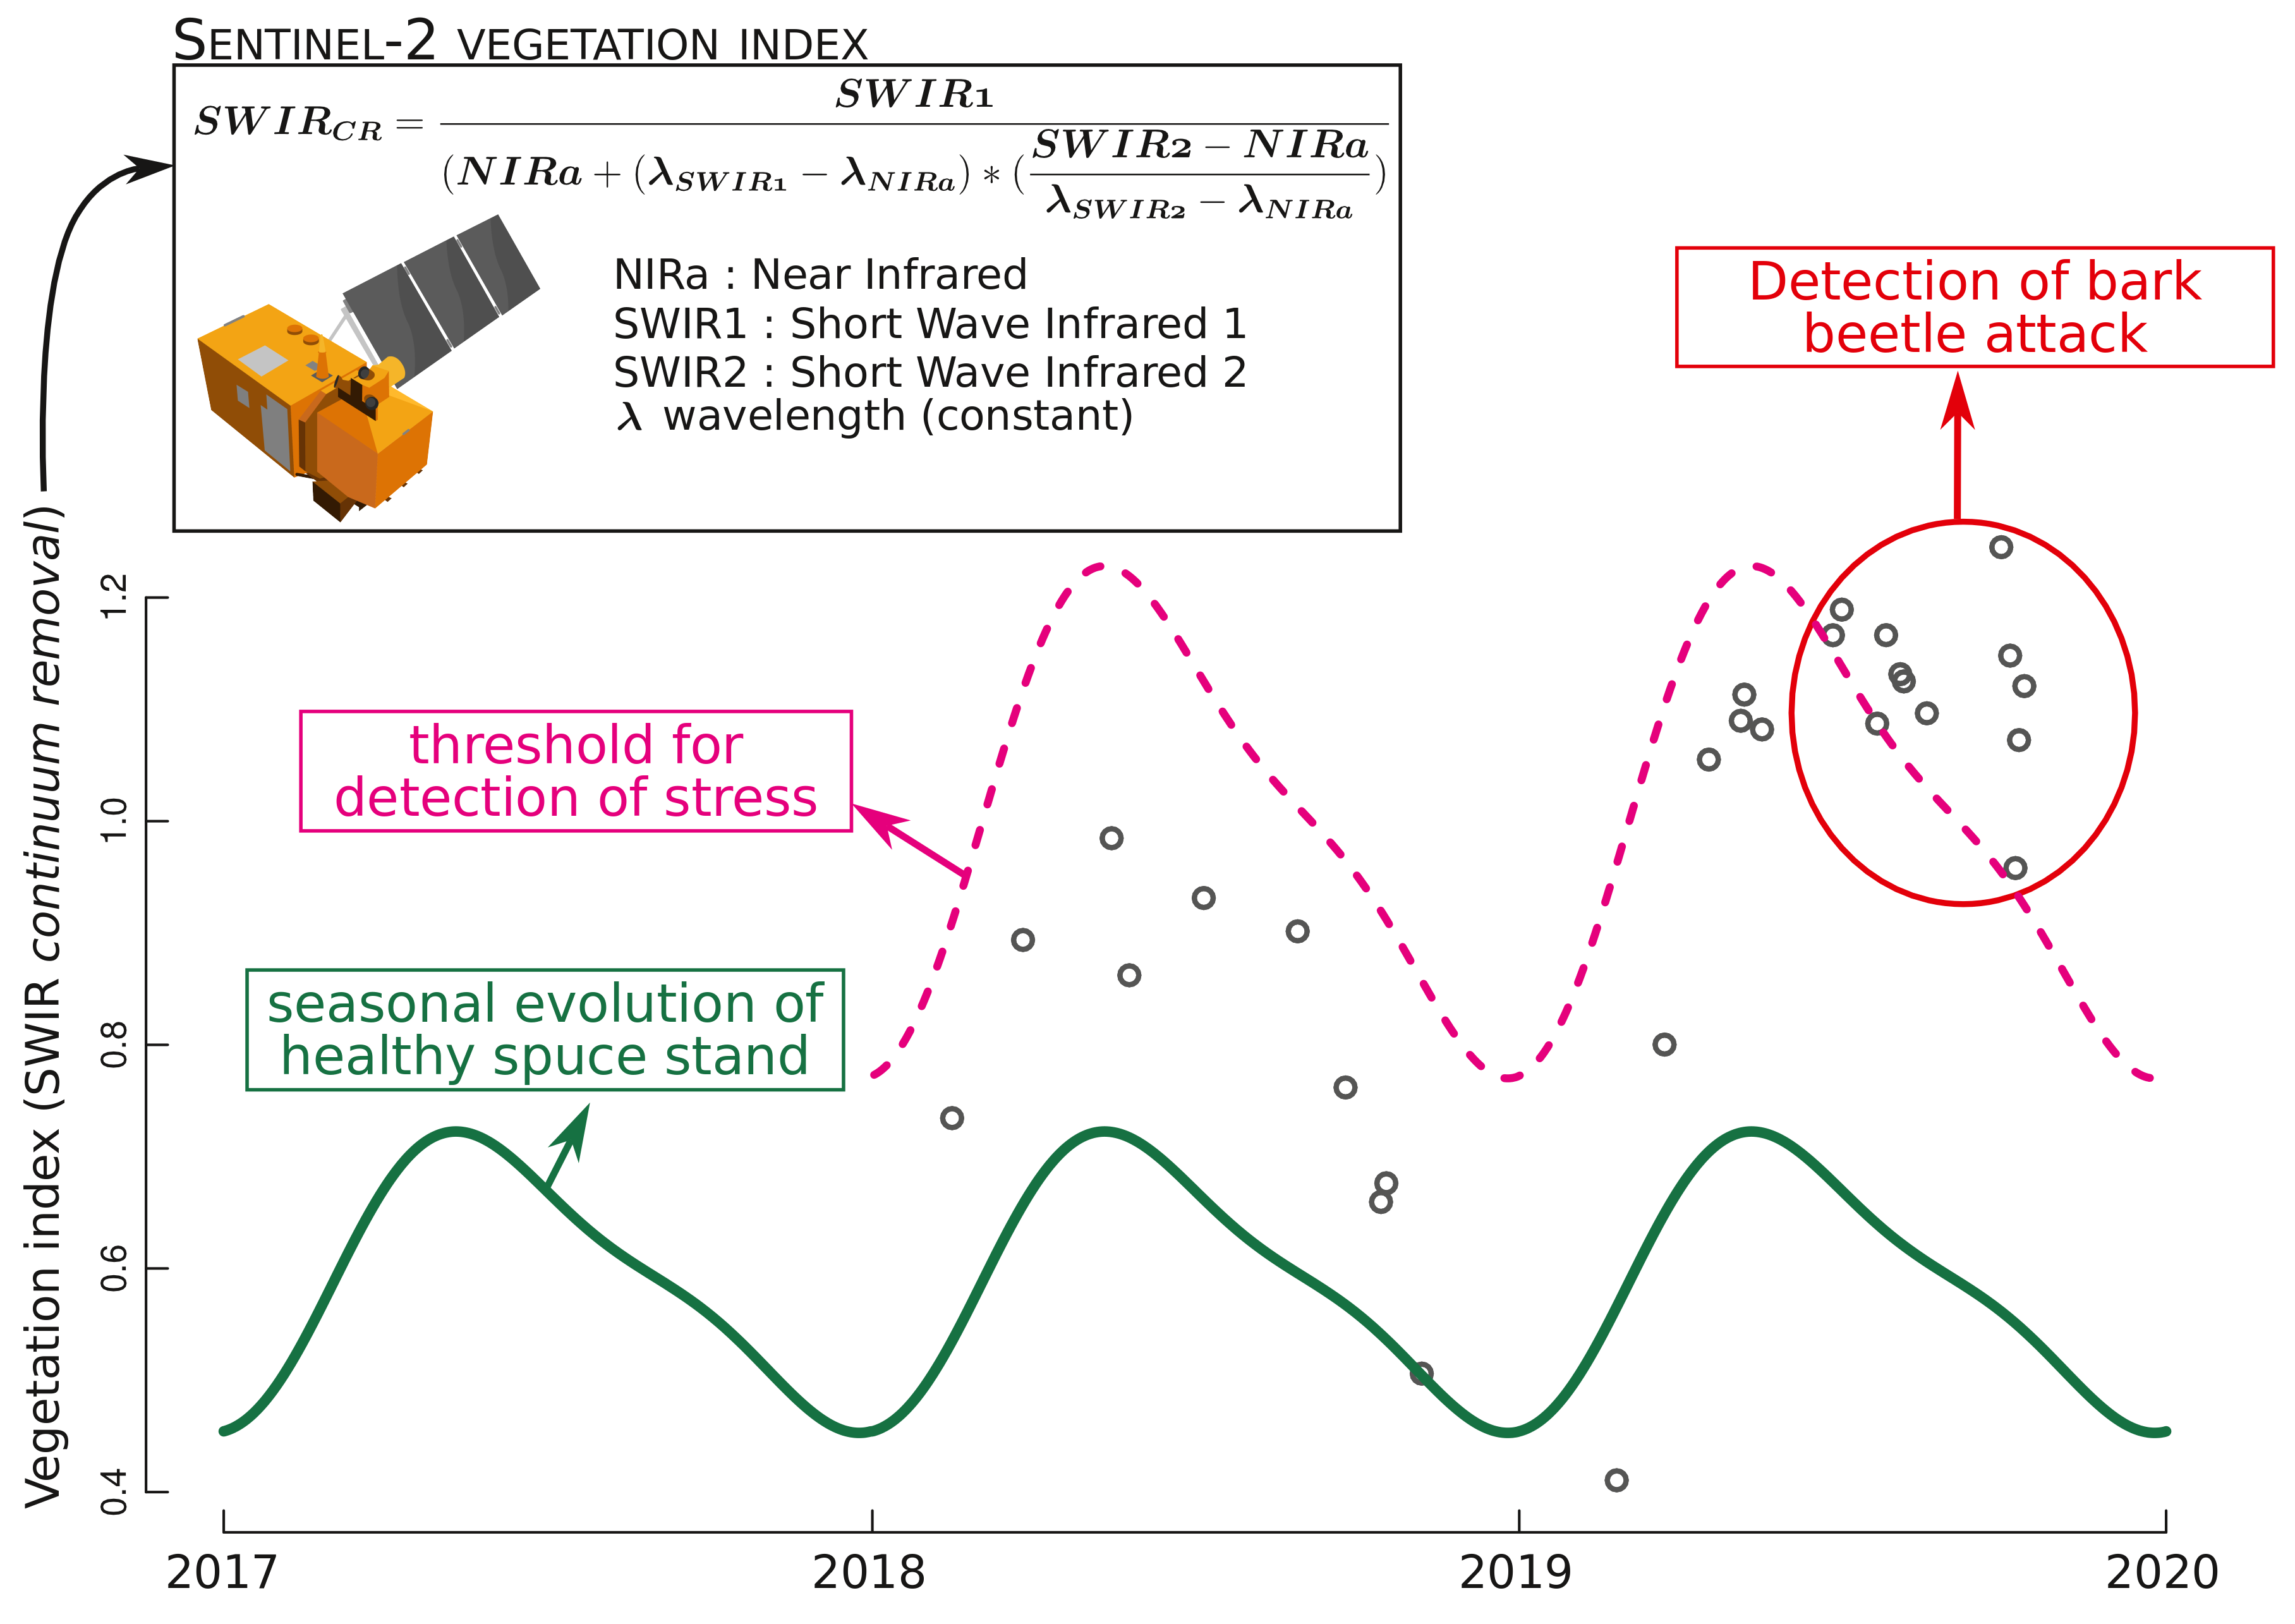
\includegraphics[width=0.8\textwidth]{fctHarmo.png}
	\caption{Bark beetle infestation map are computed by detecting change in the $SWIR_{CR}$ phenology metric. The \textit{SWIR Continuum Removal} is computed using three bands from Sentinel-2 imagery for every single acquisition date and his value is compared to a threshold (purple dashed line) in order to detect vegetation stress. If a stress is detected three consecutive times, we assume that a bark beetle infection occured.}
	\label{fig:harmo}
\end{figure}

Our approach of bark beetle detection is only suitable for spruce, as it is closely related to the phenological course of healthy spruce forest.
An essential prerequisite is thus to have a proper mapping of spruce stands.
For the south of Belgium, we use existing reliable composition maps \citep{bolyn_mapping_2022} computed from remote sensing data in order to restrict our analysis to spruces.

In the Grand-est, the composition map comes from the French Mapping agency (Forest BD version 2). 
Composition of forest stand is determined by photointerpretation and forest stands identifyed as "spruce or fir" serve as starting point to limit our analysis.
Time series are a convenient means to track phenology changes. 
More broadly than the dectection of bark beetle infestion, phenology courses are highly suitable for forest tree species discrimination \citep{lisein_discrimination_2015,grabska_forest_2019,ma_tree_2021}.
We have used S2 spectral bands courses along the vegetation season to refine the determination of species present in the area interpreted as "spruce or fir" in Vosges.
The objective is to identify and remove every area that are not spruce stand, as pixels located on others species than spruce are likely to be wrongly detected as a bark beetle attack.
All S2 spectral bands were first summarized for each of the four trimesters of the year, by simply averaging all observations occuring during the trimester.
Then, a Random Forest algorithm was trained on these synthetic intra-annual time serie to discriminate spruce from non-spruce pixels, based on a training set of observation from Belgium \citep{bolyn_forest_2018}.
Eventually, this Random Forest classifier was applied on "spruce and fir" area of Vosges and bark beetle detection was carried on only for pixels detected as spruce. 


%modif vosges by grand est



\subsection{Relation between bark beetle attack and environmental condition}

\subsubsection{Choice of important variables}

To select important variables that influence the Norway spruce dieback, we use the the random forest algorithm \citep{genuer_vsurf_2015} in Wallonia.
We apply the random forest only in Wallonia.
Individual classification trees are trained on a 500 samples of dead spruce stand of 0,25 Ha and 500 samples of healthy stand by randomly selecting a subset of explanatory variables (topographic and  climate variable).


\subsubsection{Variation of attack along important gradient}
For this study, we selected only spruce trees over 15 m and we have worked on 90 500 Ha in Wallonia and  on 73 715 ha of spruce in the Grand-est region.  
			
% Classe d'latitude
%calcul prob prese
%Comparaison entre le différents pays
%Depuis 2018, des attaques massives de scolytes tuant les épicéas frappent la Wallonie. Suite à ces évenements,les forestiers se sont interrogés sur cerains facteurs topographiques semblant avoir fortement influencé les attaques de scolytes.
%Les pessières situées en basse altitude semblent avoir été plus touché ainsi que les peuplement situé sur des versants sud.

%Pour caracteriser les attaques de scolytes, nous avons appliquer la méthode des random forest afin de selectionner les 2 facteurs topographiques influençant le plus les attaques de scolytes. CEs deux facteur sont l'altitude et les sous-radiatif. Nous avons ventilé l'altitude par classe de 100m et conservé les trois classes de sous secteurs définis par delvaux et galoux.

%Ensuite, afin de determiner les classes de ces facteurs les plus impactés par le scolyte, nous avons estimé les surfaces scolytés pour chacune des classes de chaque facteurs sur base des cartes d'état sanitaire pour chaque année de la période 2016-2021.

%La carte d'etat sanitaire de la pessière a été subdivisée en tuile de 50*50m (25 pixel de 10X10m) comprenant au minimum 17 pixel de 10mX10m d'épicéas. Une tuile est considérée comme %scolytée quand minimum 3 pixels sur 25 sont scolytés.

%Pour chaque tuile, la classe d'altitude et le sous-secteur ont été extraits.

%Nous avons calculé le ratio du nombre tuiles scolyté d'une classe divisé par le nombre total de tuiles de la classe (probabilité de présence) pour chacune des classes d'altitude et de sous-secteurs.


%\begin{align*}

%$presence\,of\,probability = \frac{tiles\, affected\, by\, the\, bark\, beetle\, of\, a\, class}{total\, number\, of\, tiles\, in\, the\, class}$

%\end{align*}



%However, other factors such as degres day data could influence bark beetle attacks 
%We made a selection of factors influencing bark beetles favourably and norway spruce unfavourably using the random forest method. The factors emerging from this analysis show that altitude and radiative topography orientation are the most important factors influencing spruce dieback  
To characterise the bark beetle attacks, we applied the random forest method to select the two topographic factors that most influenced the bark beetle attacks.
These two factors are altitude and topography orientation. We broke down the altitude by 100m classes and kept the three topography orientations classes defined by \cite{Delvaux_galoux}.
Then, in order to determine the classes of these factors most impacted by the bark beetle, we estimated the bark beetle areas for each class of each factor based on the sanitary status maps for each year of the period 2017-2021.

%The spruce health map was subdivided into 50*50m tiles (25 pixels of 10X10m) comprising at least 17 pixels of 10mX10m spruce. A tile is considered to be barked when at least 3 out of 25 pixels are barked.For each tile, elevation class, topography orientation and the sanitary status were extracted. We calculated the ratio of the number of tiles attacked by bark beetle in a class divided by the total number of tiles in the class (probability of occurrence) for each of the elevation and topography orientation classes.




%\begin{itemize}
%	\item Random forest  
	

%	\item test de student
%	\item the probability of presence of bark beetles
%The probability of bark beetle presence is the area affected by bark beetle attacks on the total spruce area. 



%Equation 
%\end{itemize}


\section{Results}

\subsection{Choice of environmental variable}
The altitude and the topographic orientation were selected as explanatory variable by the random forest algorithm.
We study the dieback of the Norway spruce in function of this two variables.



\subsection{Evolution et importance}

The drought touched the western Europe since 2018.
However, the outbreaks did not occur at the same time in the different region but the decrease of damage begin in the same year in all of our study area (Figure \ref{evol_gen}).
The first major dieback took place in the Plains in 2018.
One year later, the important damage have begun in 2019 in the Vosges and in the Ardenne.  
The area killed by this resinous pest is detailed in table \ref{tab_recap}.
%add reference crise 5 ans
The area of Norway spruce killed by bark beetle in Ardenne is 13 435 Ha.
The maximum of the ratio of area touched by bark beetles during crisis peak in 2019 is 3,4\%. 
A begin of decrease is started in 2021.

In the Vosges, there is 3218 Ha killed by bark beetle.
However, the maximum ratio of area affected by this insect is 5,5\%.
At the peak of the crisis the Vosges are proportionally more affected than the Ardenne.

The Plains group is the group with the most area and proportion of area affected.
This regions have three times more area touched by bark beetle than the Vosges.
The Plains region reached the maximum of area affected by bark beetles in 2020. 
The peak of proportion of area impacted is reached at 23,7\%.
In total, more than half of the spruce stands were affected by bark beetles in this area.

% add syrface


\begin{table}[]
 \caption{Summary table of the crisis }
 \label{tab_recap}
\begin{tabular}{|l|l|l|}
\hline
Region   & \begin{tabular}[c]{@{}l@{}}Total Norway spruce \\ area killed by bark beetle (2016-2021)\end{tabular} & \begin{tabular}[c]{@{}l@{}}Total Norway spruce \\ area before crisis\end{tabular} \\ \hline
Plains  & 13665 Ha                                                                                              & 25 552 Ha                                                                         \\ \hline
Ardenne & 13435 Ha                                                                                              & 101 600 Ha                                                                        \\ \hline
Vosges   & 3218,71 Ha                                                                                               & 26 327 Ha                                                                        \\ \hline
\end{tabular}
\end{table}




%The evolution of the crisis differs between these two neighbouring regions.

%In Wallonia, during the year 2017 and 2018, there are already norway spruce affected by bark beetle in low elevation but the probability of presence is under 10\%. 
%In 2019, the peak is reached in all of classe of elevation. During this year, the percentage of area of the Wallon norway spruce stand affected by bark beetle is 2.8\%.
%In 2020, there a  little diminution of attack. 
%During 2021, there are important diminution of area impacted by bark beetle. The probability of bark beetle presence returns to the same level as begin the crisis.

%In Grand-Est, during 2017, the attack of bark beetle are weak. 
%In 2018, there are first attack at low elevation but always below 5\%.
%In 2019, the increasing of attack at low altitude continues.
%In 2020, in all altitude classes are impacted by bark beetle. 
%Between 100m an 400m of altitude there are a important augmentation of the probability of presence. 
%The maximum of area affected is reached. % indiqué pourcentage max atteint
%During 2020, there is 4\% of the total area of spruce stand of Grand-est that area affected by bark beetle during 2020.
\begin{figure}
   \centering
   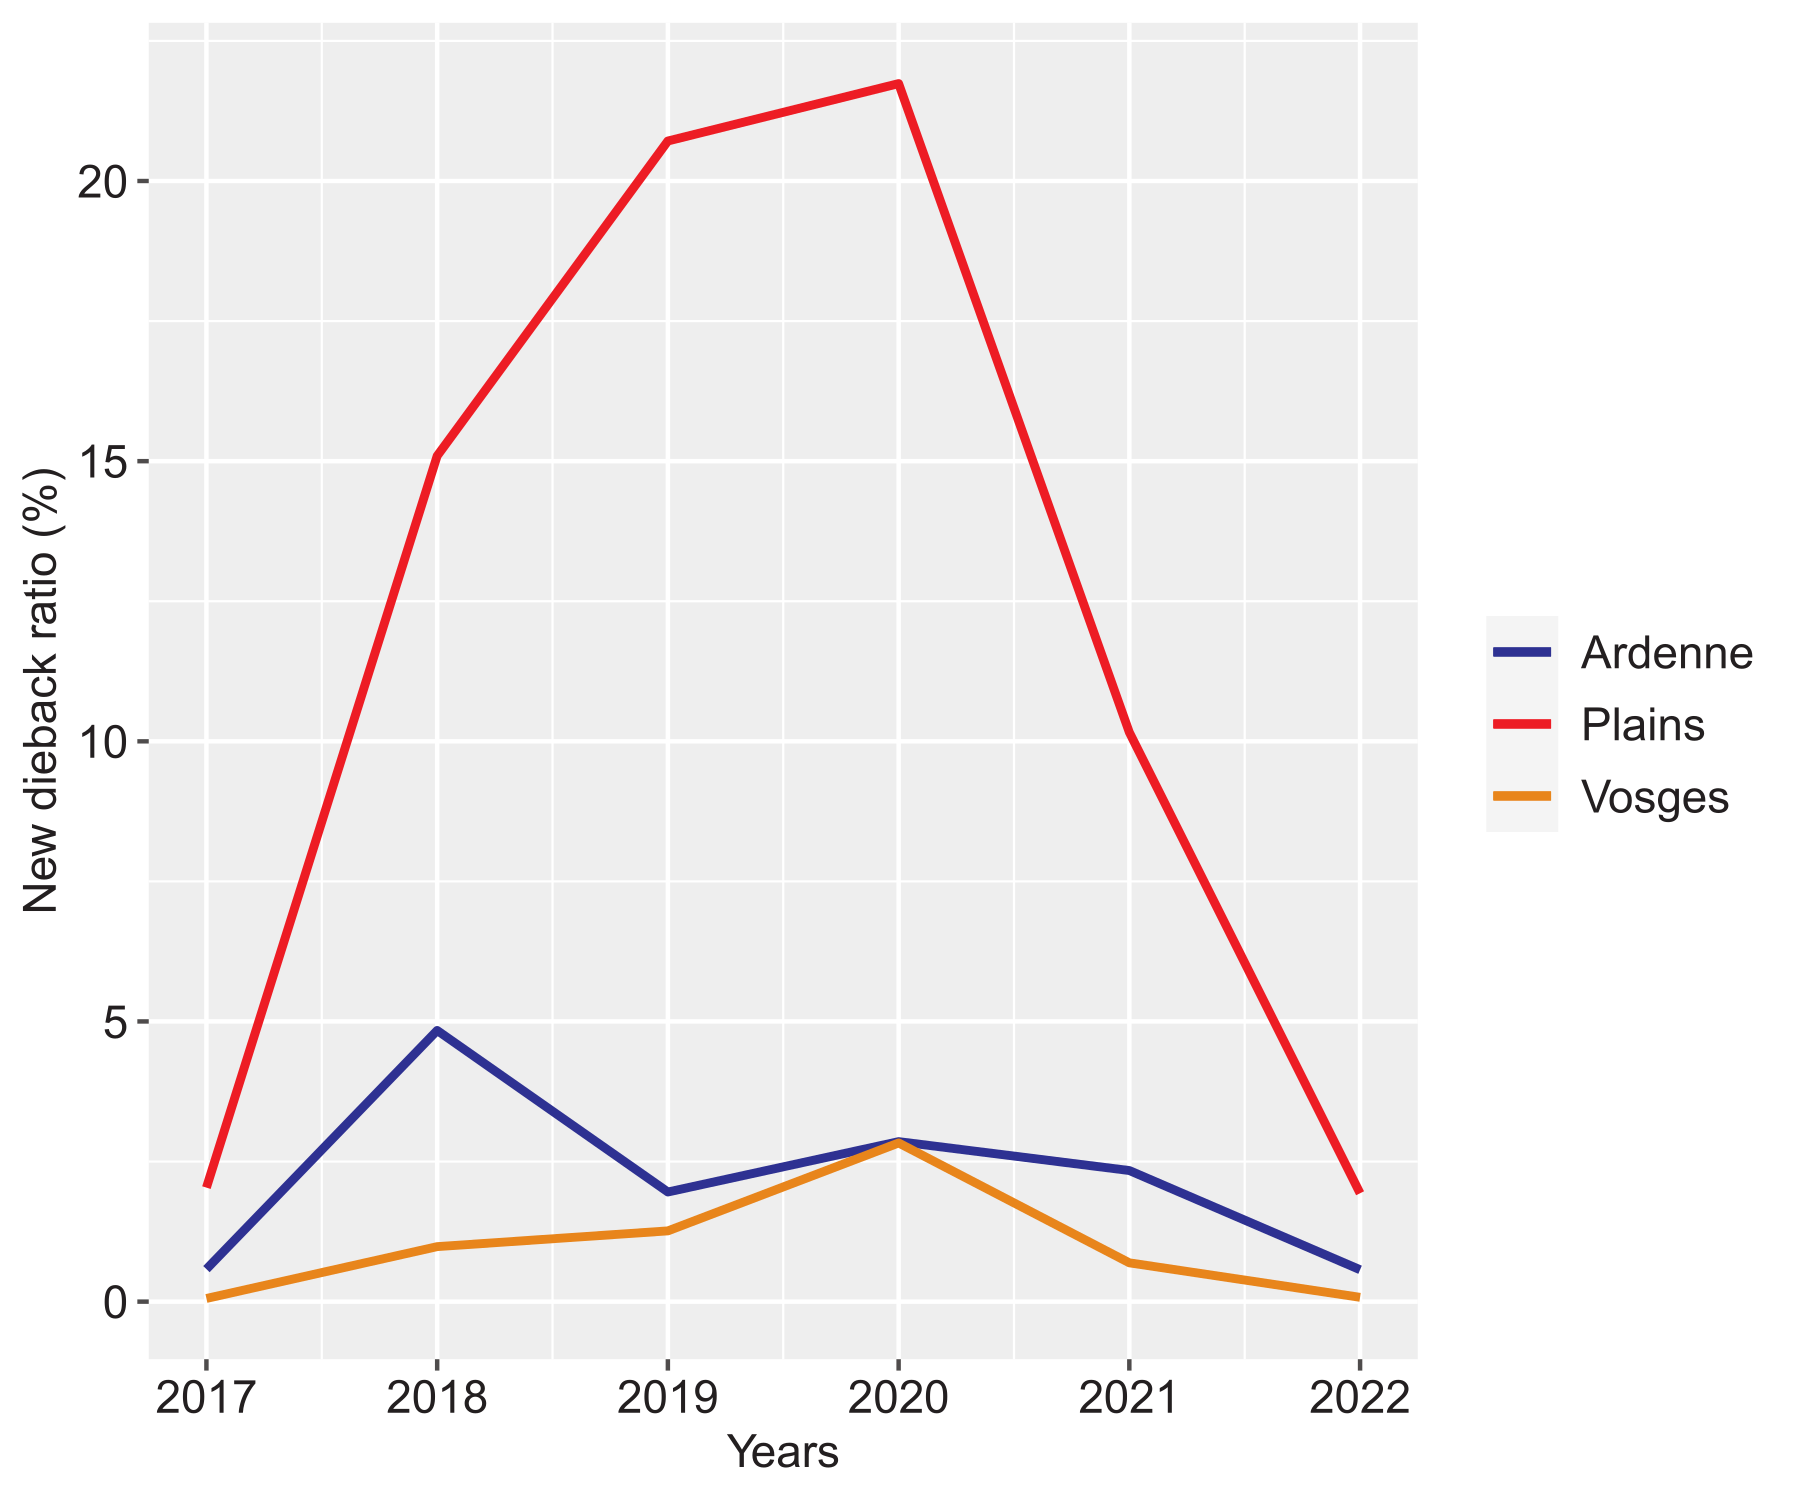
\includegraphics[width=0.6 \textwidth]{Annual_evol_Ardennes_vosges_plaines.png}
    \caption{Proportion of Norway spruce area affected by bark beetle. Plains region in red, Ardenne in blue and Vosges in }
    \label{evol_gen}
\end{figure}

    


\subsection{ Altitude vs bark beetle presence}
The altitude is easily usable for the forest manager.
The precipitation in western Europe depend of altitude. 
The majority of spruce in the Plains is located in low altitude under 400m of altitude in contrast with the Ardenne and the Vosges where the majority of Norway spruce stand grow above 400m. 
The variation of the probability of presence of bark beetles in the three groups naturals regions for the period 2017-2021 is described in the figure \ref{alti_sco}.
%The altitude has been subdivided into the same 12 elevation classes for both regions. 
%The graphs corresponding to the variation of the probability of presence in Wallonia are in the upper part of the figure and those for the Grand-Est in the lower part.

\begin{figure}
\centering
	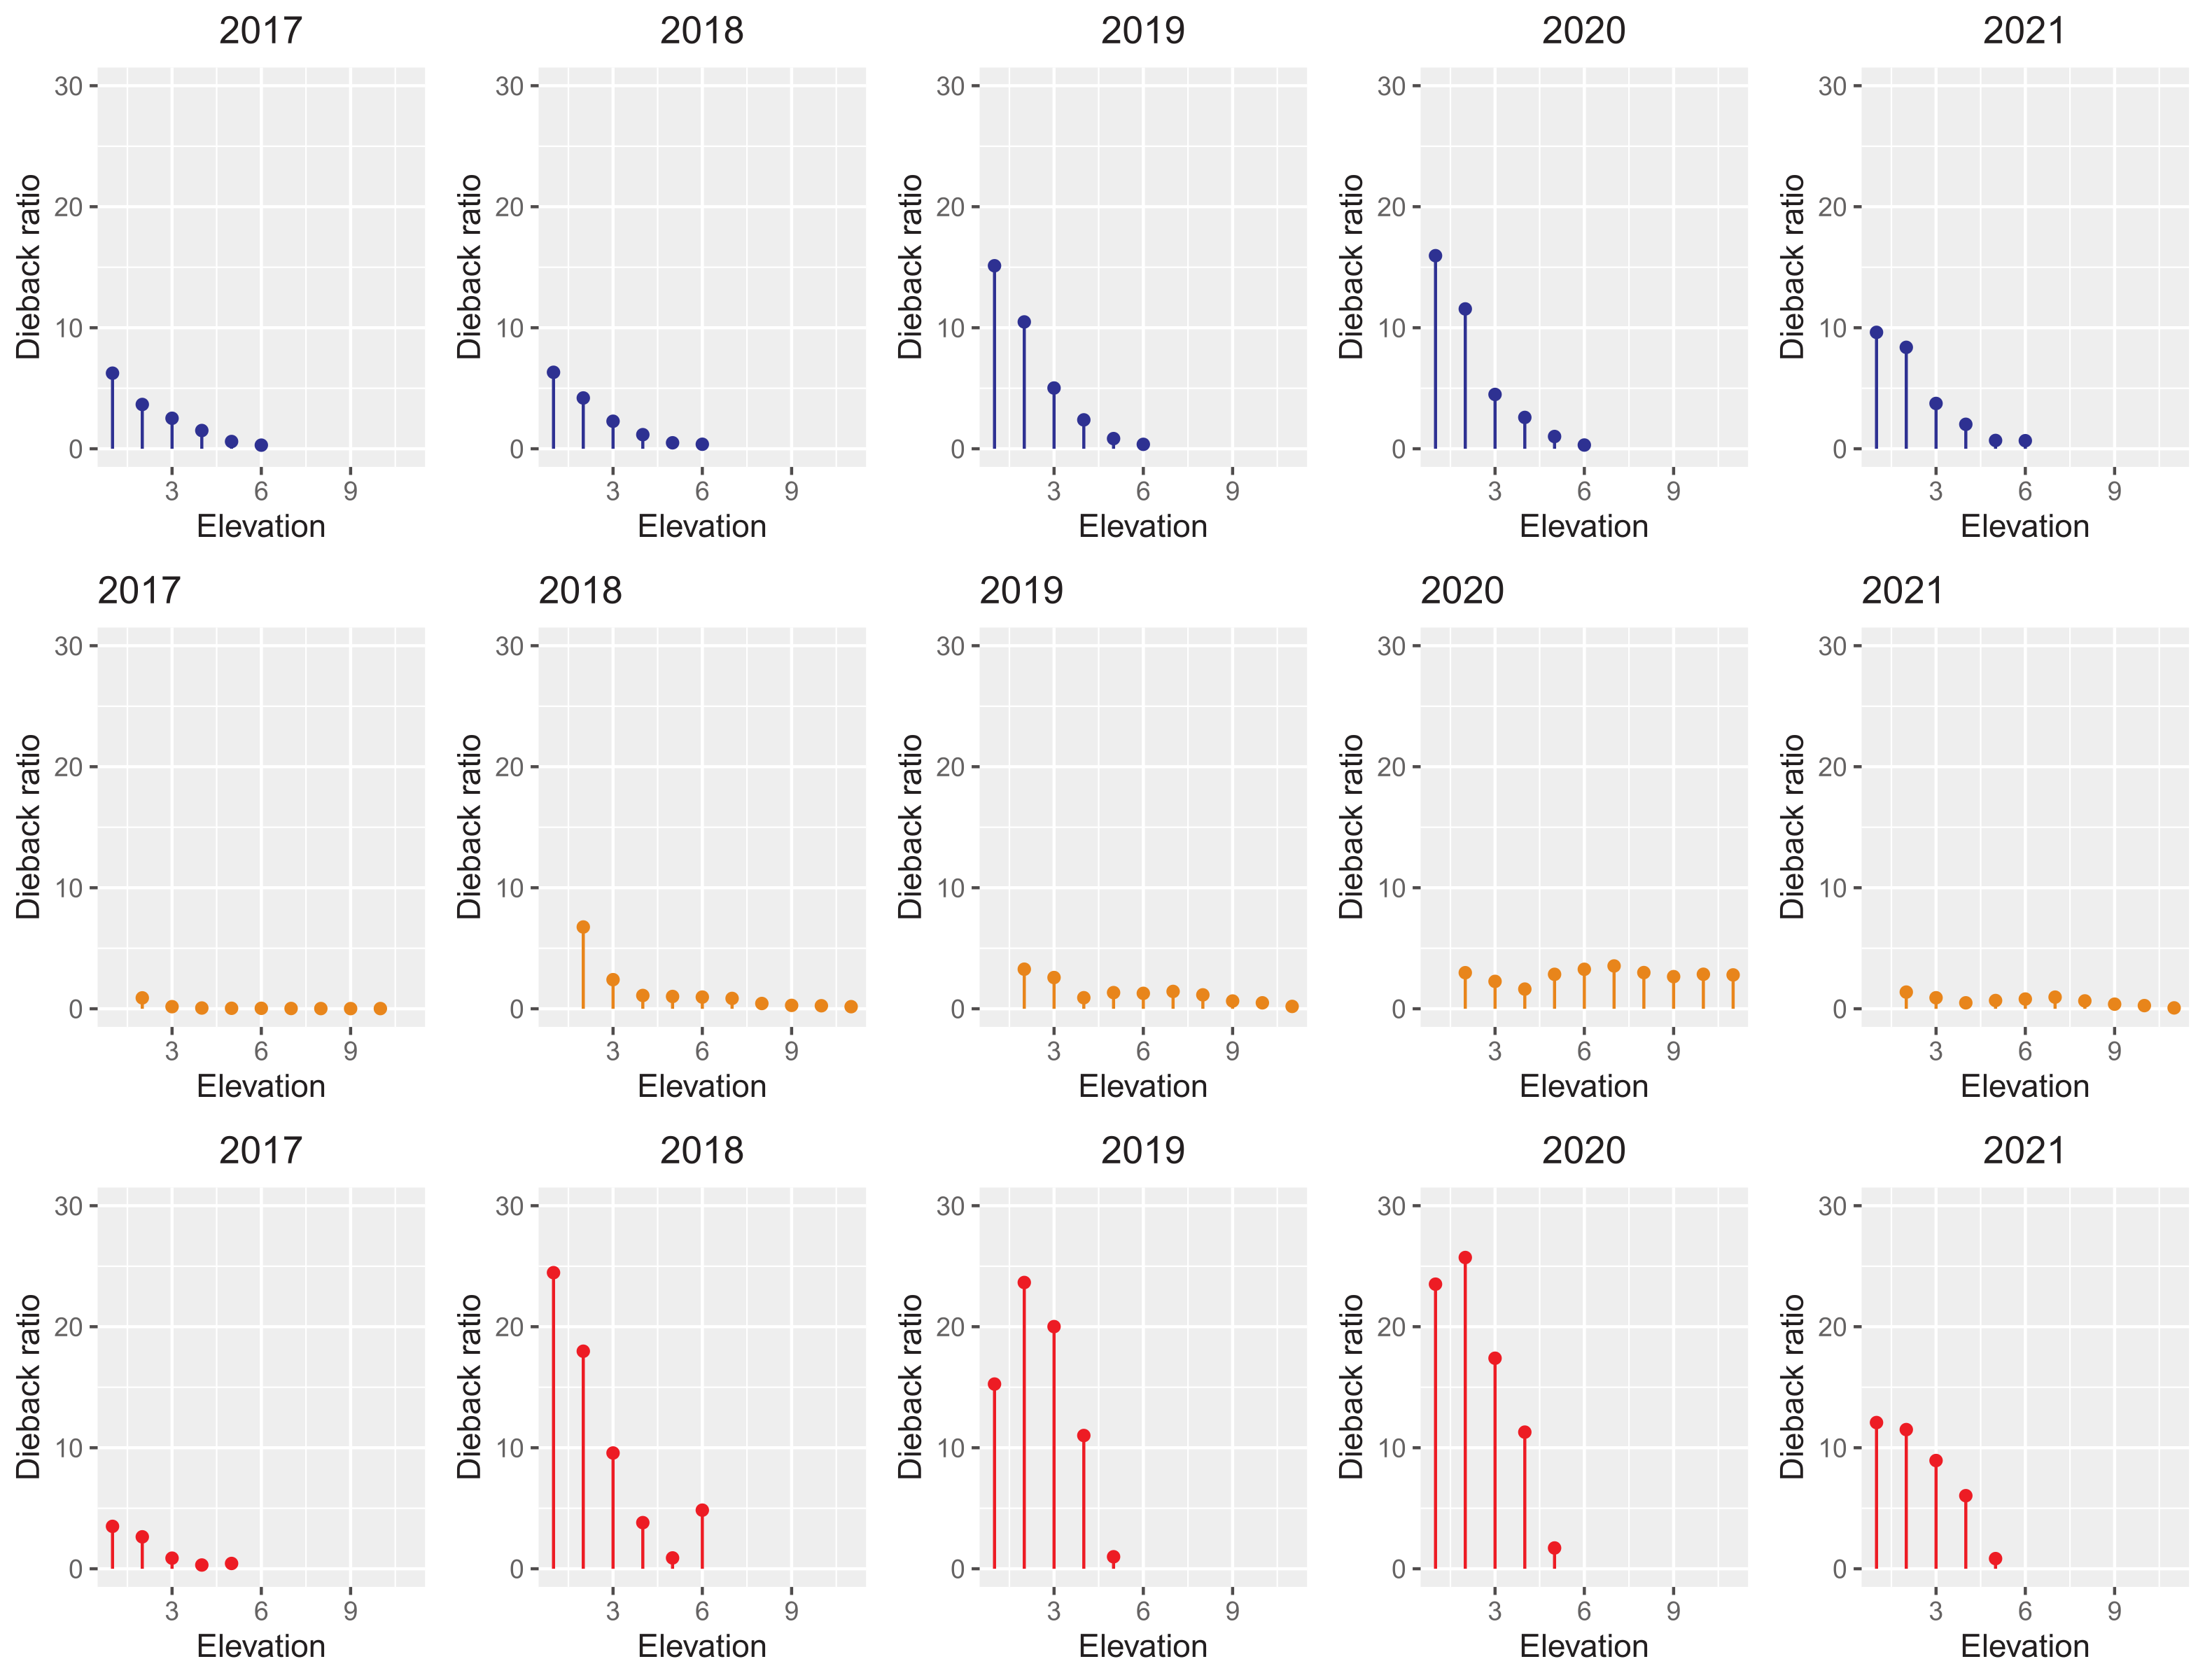
\includegraphics[width=\textwidth]{synthese_color_06_2022.png}
     \caption{The altitude has been subdivided into the same 12 altitude classes for both regions. 
The graphs corresponding to the variation of the probability of presence in Ardenne (blue) are in the upper part of the figure,the Vosges (Orange) in middle part and for the Plains (red) in the lower part.
}
	\label{alti_sco}
\end{figure}

In Ardenne group, in the begin of the crisis, the low altitude classes are more affect than hight altitude classes.
The dieback of Norway spruce occur along a altitudinal  gradient.
This gradient is confirmed over the 5 years of the study.
Indeed, during this year a strong increase in the 100-200m and 200-300m altitude classes is observed. 
These two altitude classes are more affected during this crisis.
The stand located above 400m are weakly attacked with maximum 2,5\% of presence.

In Vosges group, there are not altitude classes more affected than other. 
The low altitude are poorly represent. There are no impact of altitude on the presence of bark beetle. 
The probability of presence of this insect is inferior of 5 \% during the study period.

The Plains group are affected mainly in low altitude with a hight probability of presence of bark beetle. 
During the crisis the class of altitude 100m-200m et 200m-300m are strongly affected with a probability of presence exceeding 20\%.
There is also like in the Ardenne group, a diminution of bark beetle attack along altitudinal gradient.
The low altitude stand are the more affected stand and are disappearing.

During the five crisis year the trend are similar in the three regions, there is more attack in the low altitude classes. 

%The decrease the probabilty of bark beetle presence follow an altitudinal gradient.
%The higher the norway spruce stand grows at an altitude, the lower the probabilty of bark beetle presence. 
%For the Grand-Est region, there is an increase in the probability of bark beetle presence between 2019 and 2021. 

%In the Grand-Est stand, the situation differs than is neighbour region. In 2017, there is low presence of bark beetle  at all altitude.
%The crisis begin weakly in 2018 with attack at low altitude.
%However the probability of presence of bark beetle increase until 2020 to reach more than 20\% of norway spruce killed at altitude below 300m.
%Above 400m, the decreasing didn't follow a altitudinal gradient.
%The probability of presence of bark beetle is relatively constant with a little increase between 700-800m.
%Above 400m, the altitude didn't protect spruce against bark beetle attack in the Grand-Est.

%Unlike the Walloon spruce forest, there is no clear altitudinal gradient in the Vosges. 
%As in Wallonia, the 200-300m altitude class is strongly affected by the bark beetle. The probability of presence decreases along an altitudinal gradient between the altitude classes 200-300 and 400-500m. However, above 500m the probability of bark beetle increases up to the altitude class 700-800m.
%_Description figure \ref{fig:sco_alti} 
% augmentation de la probabilité de présence jusqu'en 2020 et diminution en 2021
% Wallonie: Diminution de la probabilité de présence de scolyte avec l'augmentation de l'altitude 
% Vosges pas de relation clair avec l'altitude. Cependant, les classes d'altitude 2, 11 et 12 semblent + touchées que les autres classes d'altitude
% et ne pas oubnlier de citer untel et machin
	
% Wallonie + Vosges: Augmentation de la probabilité de présence de scolyte avec le temps quelque soit la classe d'altitude.


\subsection{Topography orientation vs bark beetle presence}

Topography orientation influence the presence of plant and tree species. 

This is a parameter easily usable by the forest manager in the field.  

In Ardenne, from the beginning of the period to the end, the trend is the same slope are more affected by bark beetles than the plateau. 
The north and south facing slope are similarly affected until 2020. 
After 2020, the south facing slope are less impact than the north facing slope. 
The maximum of attack is reached in 2019 with 4 \% in the two orientations slopes.

The Plains group is the most affected. 
There are not clear trend for the repartition of attack on the topographic orientation.
Before 2020, the north facing slope are the most touched by bark beetles.
From 2020,the attack in the south facing slopes exceed the attack in north facing slope. 
The peak of attack is reached during this year.

Before 2019, the Vosges are weakly impacted by bark beetle. 
The plateau is more affected than the slope.
The north-facing slope are more slightly touched than the south-facing slope. 
However, in 2020 the peak of the crisis is reached. 
The plateau are always the topographic orientation the most impacted with a proportion of Norway spruce killed by bark beetle of 6,7\%.
The trend for slopes has reversed. 
The south-facing slope are more affected. 

\begin{table}[]
\begin{tabular}{|l|l|l|l|l|}
\hline
Climatic area  & Thermal sector     & \begin{tabular}[c]{@{}l@{}}Cumulative area affected \\ by bark beetle (Ha).\end{tabular} & \begin{tabular}[c]{@{}l@{}}Norway spruce area\\ before crisis (Ha).\end{tabular} & Probability of presence (\%) \\ \hline
Plains  & North-facing slope & 1592                                                                                     & 2660                                                                             & 59,8                         \\ \hline
Plains  & Plateau            & 11337                                                                                    & 21450                                                                            & 52,8                         \\ \hline
Plains  & South-facing slope & 738                                                                                      & 1442                                                                             & 51,1                         \\ \hline
Ardenne & North-facing slope & 2396                                                                                     & 14862                                                                            & 16,1                         \\ \hline
Ardenne & Plateau            & 9877                                                                                     & 79260                                                                            & 12,4                         \\ \hline
Ardenne & South-facing slope & 1165                                                                                     & 7475                                                                             & 15,6                         \\ \hline
Vosges  & North-facing slope & 1392                                                                                     & 35690                                                                            & 3,9                          \\ \hline
Vosges  & Plateau            & 1280                                                                                     & 25052                                                                            & 5,1                          \\ \hline
Vosges  & South-facing slope & 546                                                                                      & 12975                                                                            & 4,2                          \\ \hline
\end{tabular}
\end{table}

  



\iffalse\subsection{Evolution et importance}

The evolution of the crisis differs between these two neighbouring regions. 
In Wallonia, during the year 2017 and 2018, there are already Norway spruce affected by bark beetle in low altitude but the probability of presence is under 10\%. 
In 2019, the peak is reached in all of classe of altitude. During this year, the percentage of area of the Wallon Norway spruce stand affected by bark beetle is 2.8\%.
In 2020, there a  little diminution of attack. 
During 2021, there are important diminution of area impacted by bark beetle. The probability of bark beetle presence returns to the same level as begin the crisis.

In Grand-Est, during 2017, the attack of bark beetle are weak. 
In 2018, there are first attack at low altitude but always below 5\%.
In 2019, the increasing of attack at low altitude continues.
In 2020, in all altitude classes are impacted by bark beetle. 
Between 100m an 400m of altitude there are a important augmentation of the probability of presence. 
The maximum of area affected is reached. % indiqué pourcentage max atteint
During 2020, there is 4\% of the total area of spruce stand of Grand-est that area affected by bark beetle during 2020.

\fi
 
  




\section{Discussion}

\subsection{Global trend}

In the current study, we found that the plains natural region is most sensible at the attack of bark beetles.

In this natural region, the proportion of attack in 2017 is already over 4 \%. 
This proportion is superior at all maximum of two others regions. 
The bark beetle is already present in this region because the climate in 2016 was favourable for the development of bark beetle. 
In fact, the sales data of Department of nature and forest of Wallonia show a increasing volume of Norway spruce infested by bark beetle.
The plains region is warmer and with less precipitation than the two others regions.
The climate condition are suitable for the multiplication of generation of bark beetle during the year (\citep{baier_phenipscomprehensive_2007} and \citep{annila_influence_1969}).

The first major attack of bark beetle have started in the plains in 2018 but the majority of the damage occurred in 2019. 
The explosion of the ratio of area impacted by bark beetle can be also explain by a non-proactive management of forest in this area.

%Bof
The sanitation felling allow to limit explosion of bark beetle \citep{stadelmann_effects_2013}.
The plains region is not a resinous region and the resinous sawmill are far the forest. 
The time between the infestation of the stand and the sanitation felling is probably to long and allow more easily a pullulation of bark beetle.
%According to \citep{dobor_spatial_2020}, a salvaging intensity below 80 \% impact the bark beetle disturbance.  

In Ardenne, the peak is reached in 2019. The maximum is 4 \%. The climate of ardenne is more suitable for Norway spruce. 
%This climate is nearby mountain climate. 
The climate can explain a the limitation of damage in region. 
The air masses come to call on the Ardenne massif and important precipitations are created following a foehn effect, allowing the spruce to suffer less from the drought in this region at low altitudes compared to the Vosges massif. 
%cite etude climato
At similar altitudes, this foehn effect allows the Ardenne spruce to be less affected by drought than the spruces of the plains.

In the Vosges, the increasing of area impacted by bark beetles is relatively weak.
The Norway spruce os a endemic species in the Vosges mountain. 
The moutain climate protect this resinous species. 
Besides the vosgian forest is generally mixed with beech (\textit{Fagus sylvatica}) and  silver fir (\textit{Abies alba}). Mixed forest are significantly more resitant to pest attack \citep{jactel_2021}. 

The difference of proportion affected by bark beetle in Ardenne and Vosges can be expained by type of forest.
In Ardenne, the even aged pure stand is predominantly whereas in the Vosges  the forest are more mixed. 

\subsection{Altitude}


The Norway spruce is a tree species naturally present on the top of the Vosges mountain \citep{guinier_trois_1959}. 
It was introduced in the low altitude Vosges and in  all part of the Ardenne and the Plains. 



 






All of spruce species need important amount of water. 
In the Plains, all classes of altitude are touched more than 10 \% during the crisis except for the classe 500-600m. 
The altitude didn't protect the tree during the drought. 
All of this stand are artificial stand plant in area not adapted for mountain tree. In the Ardenne from 300m to 700m the forest have been affected to a maximum of 5\%. 

The weak damage can be explain by increase precipitation with altitude (\cite{kotlarski_elevation_2012}, \cite{Roe_orographic_preicpitation_2005}).
The Norway spruce is less stressed in hight altitude than in low altitude. 
The beetle can also affect by this increase of precipitation to swarm. 

Besides, in low altitude the temperature are higher than in hight altitude. 
The number of generation depend of the temperature.
And thus higher temperature produce more damage cause by the the supplementary generation. 

The altitude influence the choice of the place of overwintering of  bark beetle.
The quantity of bark beetle that overwinters under the bark decrease with altitude \citep{kasumovic_overwintering_2019}.
The litter insulate better the beetle of the freeze \citep{lombardero_cold_2000} than the bark.
However, the metabolism of bark beetle need energy from 5°C  \citep{kostal_physiological_2011}.
%faut checker car source dolezal unpublished)

% scolyte + hibernation sous écorce en basse altitude pour pouvoir se nourrir si + de 5°c en hiver donc si 




\begin{itemize}
	\item Différence climat (Climat semicontinental/montagnard vs climat tempéré océanique)
	\item Différence sylvicole ( Wallonie futaie régulière exploitable vs Vosges peuplement + mélangé et moins exploitable en haute altitude)
	\item Sommet des vosges epicéas endémiques vs épicéas en plantations (résilience peuplement )
	\item adaptation ep à condition plus rude en versant sud que nord 
	D'après la theorie il devrait y avoir plus de generation sur versant sud car car + chaud et donc pluys touché
	Seuil letal ou the letargie atteint en versant sud?
\item meilleur surveillance des forestiers sur versant sud que nord 
	
\end{itemize}

\subsection{Topography orientation}

%citer auteur versant sud + touché

The orientation of slope influence the presence of vegetation. The north facing slope receive less radiation than south facing slope. 
The life cycle of the bark beetle is influenced by temperature (\cite{baier_phenipscomprehensive_2007}, et ...). South facing slope are warmer than north facing slope.
Bark beetle make more generation of bark beetles in this area \cite{}. 
However in France, \cite{nardi_drought_2022} show that steep slopes and soils with low water availability are less attacked. 

In our study, we found that in the Vosges the slope are less impacted than the plateau. 
For the year 2019, we have the same result that \cite{nardi_drought_2022}. 
The south facing slope are less affected than the north. 
However, in 2020, the trend has been reversed the south slope are more affected than the north slope. 
This change is likely to have occurred with the increase of stress with a third dry summer in 2020.

In the plains, before 2020, the north facing slope are also more affected than the others topography orientations. 
Nevertheless, in 2020 there is a inversion of the trend. 
The south-facing slope are the most impacted and north facing slope the less.

In Ardenne, the slope are more affected than the plateau. The plateau are probably less affected because the major part of the plateau are located above 400m of altitude.
Moreover, this area stay cold in the summer and limit the number of generation of bark beetles and the stress of Norway spruce.
The north-facing and south-facing slope are similarly affected until 2021. 


 
\iffalse
\subsection{Facteur déterminant l'attaque par l'épicéa ou le scolyte}

\begin{itemize}
	\item Discussion généralisation de modèle scolyte/ dépérissement des épicéas
    \item est ce la Biologie du scolyte/ ou le stress de l'épicéa qui conditionne le dépérissement massif ?
	
\end{itemize}
\fi
\subsection{Potential limitations}
The detection of bark beetle attack is based on Sentinel 2 satellite imagery.
The methodology use Norway spruce mask. 
In pure even aged Norway spruce, the method works well. 
However, in mixed forest, the Norway spruce mask is less accurate than in pure even aged.
In fact, our sanitary map resolution is 10m and if there some deciduous tree or others resinous in the Norway spruce mask, there is a risk of error.
In Ardenne and in the Plains, there is principally pure even aged stand of Norway spruce but in the Vosges the stand are more mixed.
In this region, there is more risk of presence of beech and silver fir in our Norway spruce mask.

We overestimated probably the Norway spruce area in the Vosges region.
\section{Conclusion and perspective}

In the context of global change, the forest manager need to adapt its silvicultural choices.
In our study, we try to identify wich are the topographical variable that influence the dieback of Norway spruce.
In this study, we show that it is very risky to make new plantation of Norway spruce at low altitude below 400m in the three regions.
In the Ardenne, we recommend the plantation of this tree species on the plateau and in the Vosges on slopes. 
%We advise against the planting of norway spruce in the plains region. 
Our data does not support the new plantation of Norway spruce in Plains. 
%Dans des régions très proches, les stations de dépérissement de l'épicéa sont différentes.
%Il semble donc difficle de généraliser des modèles basé sur des relations topographique à une grande échelle. 
\section{Figure}


	

%\begin{figure}[htbp]
%	\begin{minipage}[b]{1 \linewidth}
%		\centering
	%	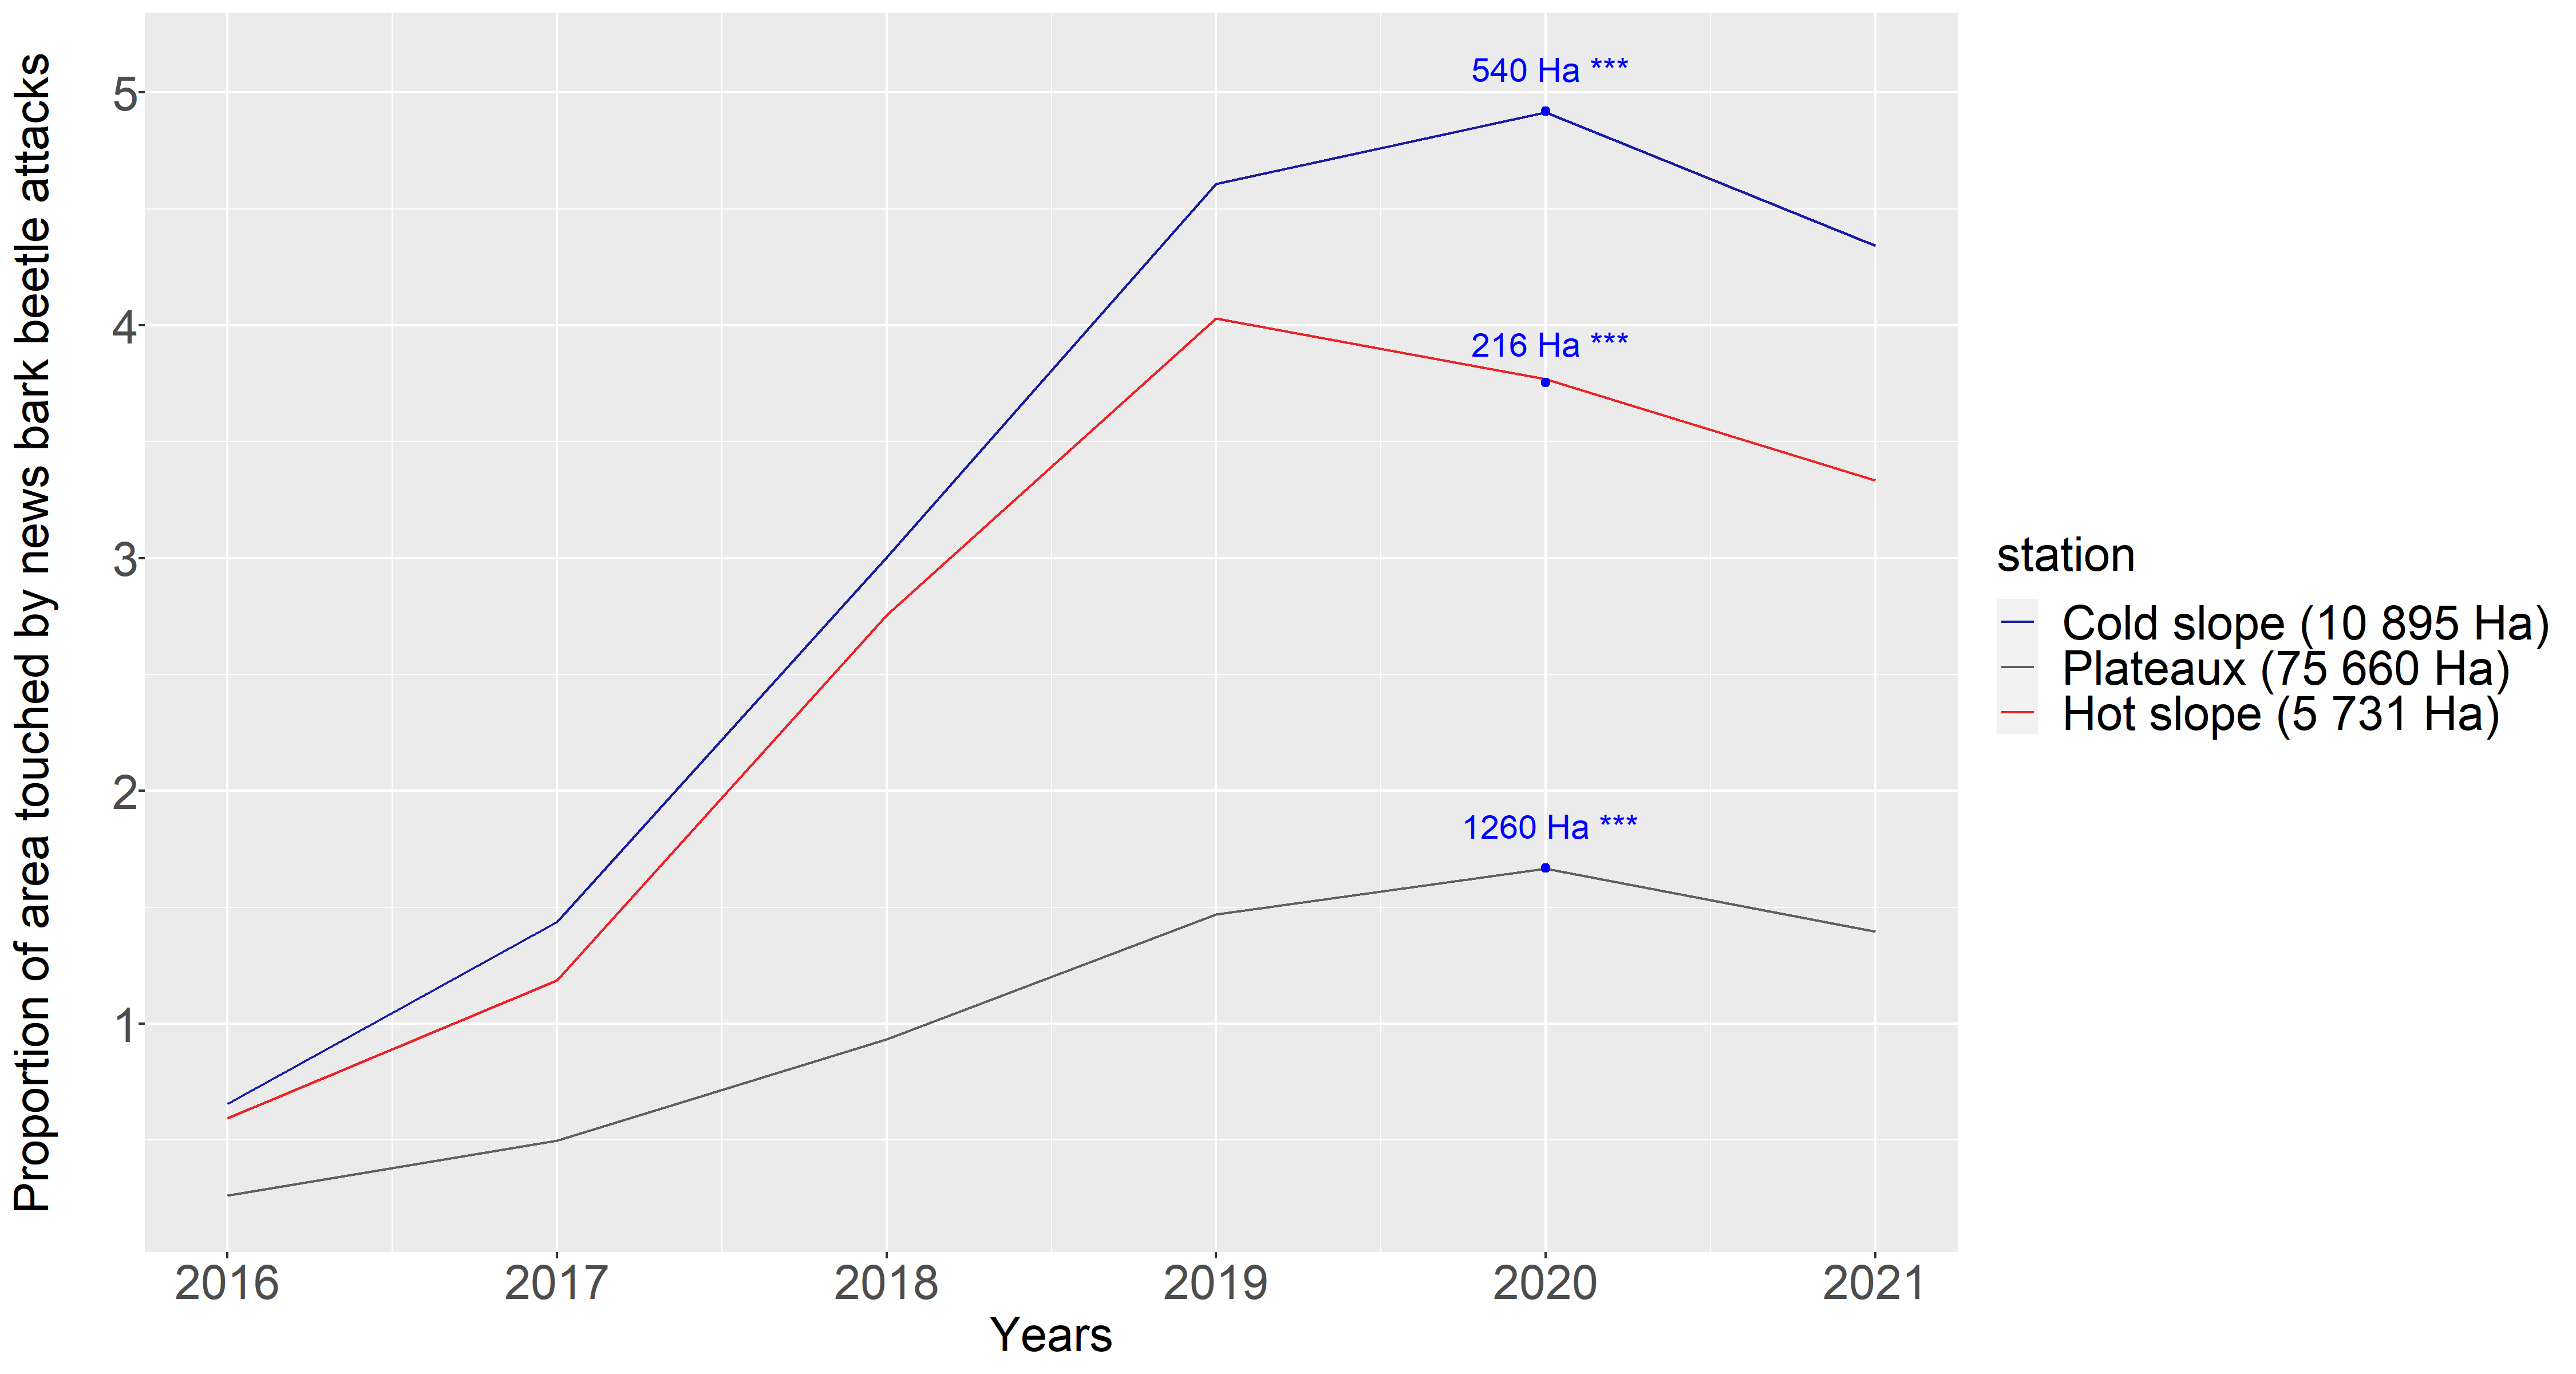
\includegraphics[width=1\textwidth]{evol_ss_wal.png}
%		\caption{Évolution de la crise du typographe en région wallonne en fonction des sous-secteurs.}
%		\label{fig:ss_wall}
		%\caption sert à insérer une légende
%	\end{minipage}\hfill
%	\vspace{1cm}
%	\begin{minipage}[b]{1 \linewidth}
%		\centering
%		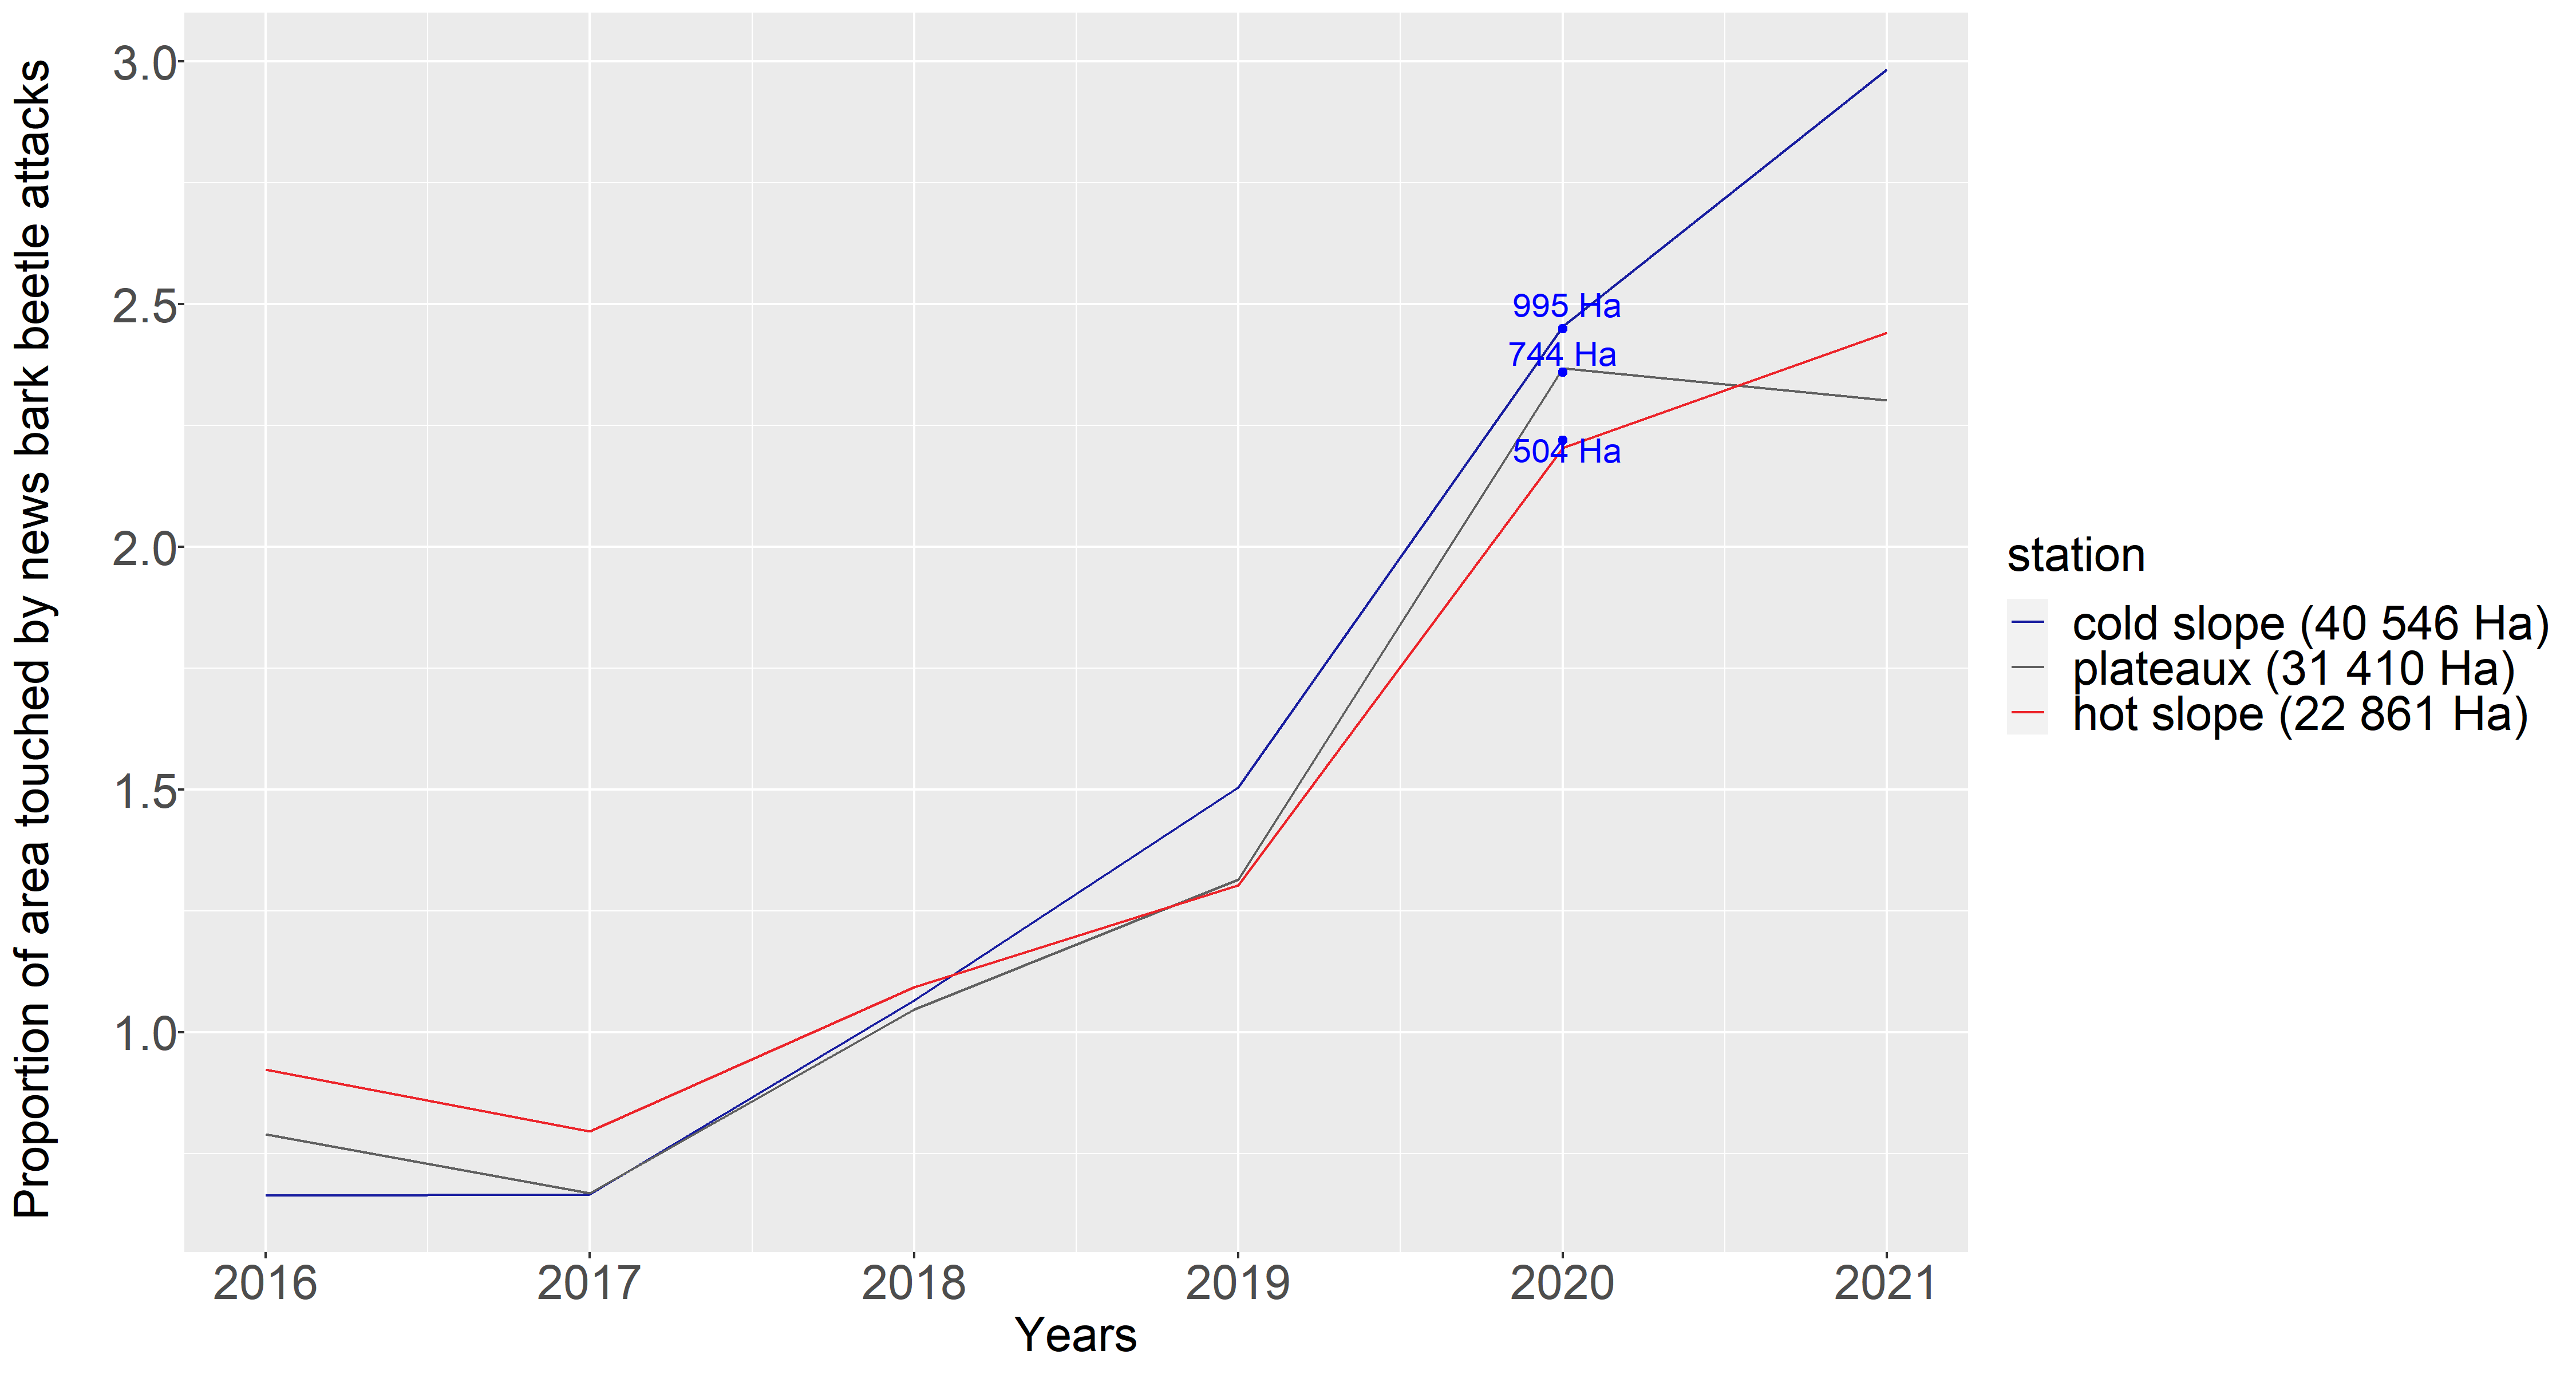
\includegraphics[width=1\textwidth]{evol_ss_vosges.png}
%		\caption{Évolution de la crise du typographe dans les Vosges en fonction des sous-secteurs .}
%		\label{fig:ss_vosg}
%	\end{minipage}
%end{figure}

\section{Acknowledgements}

This research has been funded thanks to the \textit{RegioWood II} project.

%\bibliographystyle{elsarticle-num}
\bibliographystyle{plainnatGL_v2}\biboptions{authoryear}
\bibliography{Scolyte.bib}
\end{document}